%%% LaTeX Template: Two column article
%%%
%%% Source: http://www.howtotex.com/
%%% Feel free to distribute this template, but please keep to referal to http://www.howtotex.com/ here.
%%% Date: February 2011

%%% Preamble
\documentclass[	DIV=calc,%
							paper=a4,%
							fontsize=12pt,%
							onecolumn]{scrartcl}	 					% KOMA-article class

\usepackage{lipsum}													% Package to create dummy text
\usepackage[brazil]{babel}										% English language/hyphenation
\usepackage[protrusion=true,expansion=true]{microtype}				% Better typography
\usepackage{amsmath,amsfonts,amsthm}					% Math packages
\usepackage[pdftex]{graphicx}									% Enable pdflatex
\usepackage[svgnames]{xcolor}									% Enabling colors by their 'svgnames'
\usepackage[hang, small,labelfont=bf,up,textfont=it,up]{caption}	% Custom captions under/above floats
\usepackage{epstopdf}												% Converts .eps to .pdf
\usepackage{subfig}													% Subfigures
\usepackage{booktabs}												% Nicer tables
\usepackage{fix-cm}													% Custom fontsizes
\usepackage[utf8]{inputenc}
\usepackage[top=2.5cm, bottom=2.5cm, left=2.5cm, right=2.5cm]{geometry}
\usepackage[ddmmyyyy]{datetime}
\usepackage{float}
\addto\captionsenglish{%
	\renewcommand\tablename{Tabela}
	\renewcommand\figurename{Figura}
} 
 

 
%%% Custom sectioning (sectsty package)
\usepackage{sectsty}													% Custom sectioning (see below)
\allsectionsfont{%															% Change font of al section commands
	\usefont{OT1}{phv}{b}{n}%										% bch-b-n: CharterBT-Bold font
	}

\sectionfont{%																% Change font of \section command
	\usefont{OT1}{phv}{b}{n}%										% bch-b-n: CharterBT-Bold font
	}



%%% Headers and footers
\usepackage{fancyhdr}												% Needed to define custom headers/footers
	\pagestyle{fancy}														% Enabling the custom headers/footers
\usepackage{lastpage}	

% Header (empty)
\lhead{}
\chead{}
\rhead{}
% Footer (you may change this to your own needs)

%% ====================================
%% ====================================
%% Projeto de rede ADAPAR, SEAB e EMATER
%% ====================================
%% ====================================

\lfoot{\footnotesize \texttt{Cabeamento estruturado} \textbullet ~ SEAB, ADAPAR e EMATER}


\cfoot{}
\rfoot{\footnotesize página \thepage\ de \pageref{LastPage}}	% "Page 1 of 2"
\renewcommand{\headrulewidth}{0.0pt}
\renewcommand{\footrulewidth}{0.4pt}



%%% Creating an initial of the very first character of the content
\usepackage{lettrine}
\newcommand{\initial}[1]{%
     \lettrine[lines=3,lhang=0.3,nindent=0em]{
     				\color{DarkGoldenrod}
     				{\textsf{#1}}}{}}



%%% Title, author and date metadata
\usepackage{titling}															% For custom titles

\newcommand{\HorRule}{\color{DarkGoldenrod}%			% Creating a horizontal rule
									  	\rule{\linewidth}{1pt}%
										}

\pretitle{\vspace{-30pt} \begin{flushleft} \HorRule 
				\fontsize{50}{50} \usefont{OT1}{phv}{b}{n} \color{DarkRed} \selectfont 
				}

%% ====================================
%% ====================================
%% mude o titulo  do projeto
%% ====================================
%% ====================================

\title{Projeto de cabeamento estruturado para SEAB, ADAPAR e EMATER de Ponta Grossa - PR}					% Title of your article goes here

%% ====================================



\posttitle{\par\end{flushleft}\vskip 0.5em}

\preauthor{\begin{flushleft}
					\large \lineskip 0.5em \usefont{OT1}{phv}{b}{sl} \color{DarkRed}}
\author{Marcelo Neumann e Roberto Henrique Tonete }  	% Author name goes here


\postauthor{\footnotesize \usefont{OT1}{phv}{m}{sl} \color{Black} 
					\\Universidade Tecnológica Federal do Paraná - Câmpus Cornélio Procópio 								% Institution of author
					\par\end{flushleft}\HorRule}

\date{}																				% No date




%%% Begin document
\begin{document}
\maketitle
\thispagestyle{fancy} 	
\thispagestyle{empty}		% Enabling the custom headers/footers for the first page 
% The first character should be within \initial{}


\begin{figure}
	\centering
	
\includegraphics{utfpr}
\end{figure}

\vspace{2cm}
\centerline{\textit{\textbf{\today}}}



%% ====================================
%% ====================================
%% mude o resumo  do projeto
%% ====================================
%% ====================================



%%\initial{E}\textbf{Este projeto tem o propósitvo de criar um cabeamento estruturado para a sede dos 03 órgãos do Estado do Paraná: SEAB, ADAPAR e EMATER. Este é um projeto real com poucas chances de ser implantado feito para fim didáticos da disciplina de Cabeamento estruturado. Será realizado o levantamento da planta física, elaboração da planta lógica, equipamentos passivos de rede, Levantamento de quantidade de equipamentos, plano de Certificação e orçamento.
%%	Este modelo exemplifica como um projeto de cabeamento estruturado deve ser elaborado. No projeto real,
%%	esta seção deve indicar qual seria o propósito do projeto: reestruturar, criar uma estrura sem uma anterior, apresentar uma estrutura ficticia ou real  etc. Deve também conter sua cobertura (quais elementos este projeto aborda): Levantamento da planta física, Elaboração da planta lógica, Equipamentos passivos da rede (memorial descritivo), Levantamento de quantidade/custo, Plano de Certificação e orçamento.
	%%No caso de projetos reais, deve conter também o escopo. No projeto real deve conter quais as atividades serão executadas e quais os responsáveis. Deve apresentar também as restrições que serão cumpridas e um possível acordo de nível de serviço (SLA). 	esumo pode ser descrito no formato texto ou em forma de um mapa mental/conceitual conforme figura \ref{fig4}.}


%% ====================================
\begin{figure}[h]
	\centering
	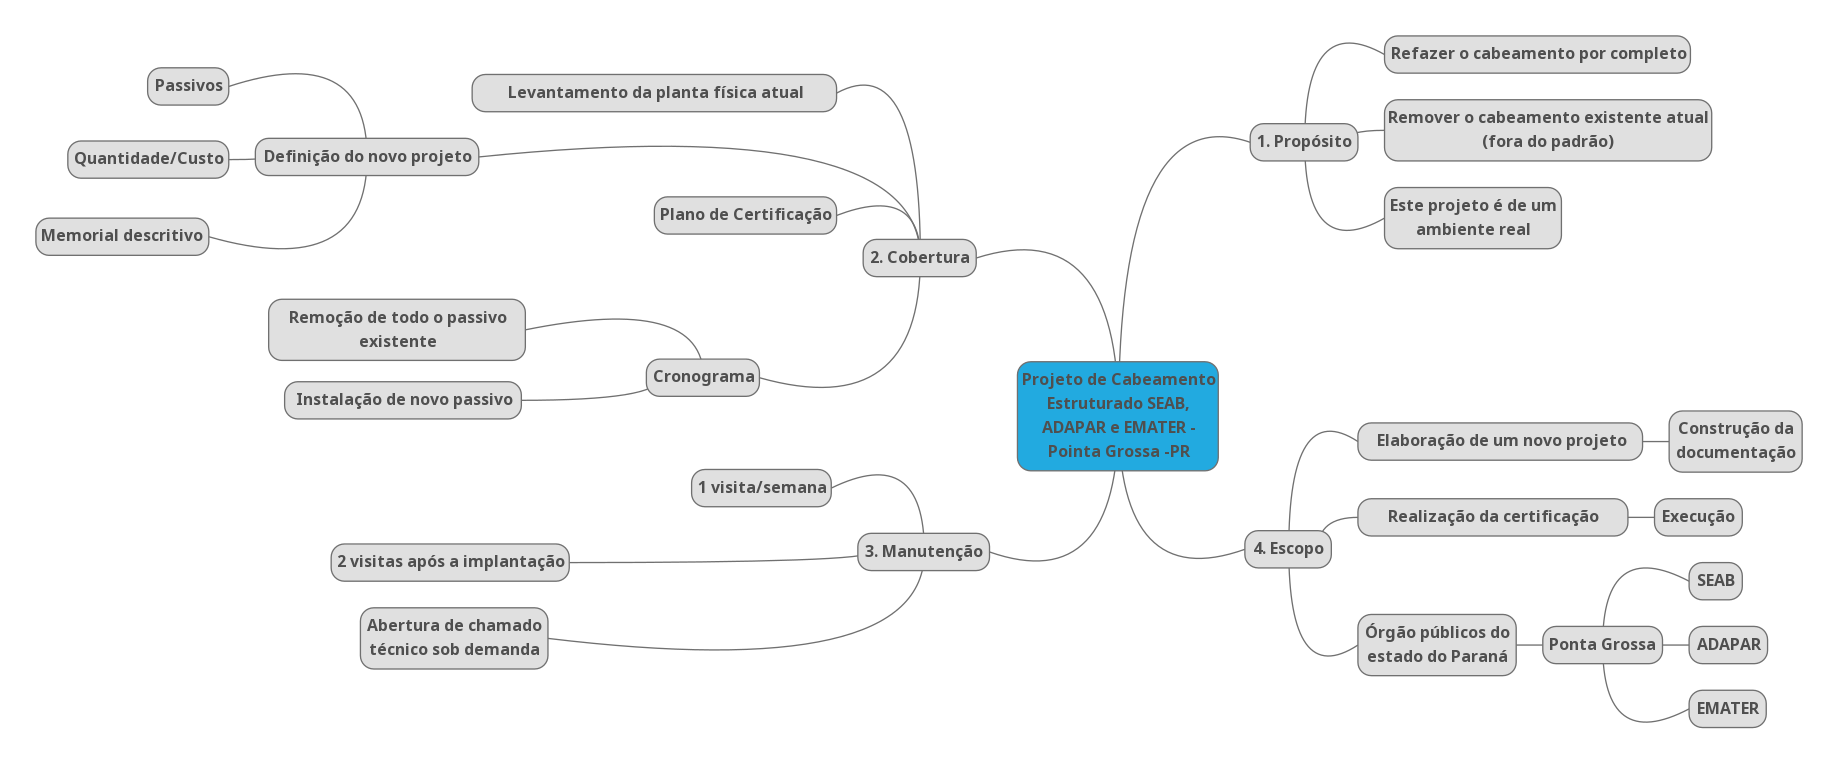
\includegraphics[height=\textwidth,width=25cm,angle=-90,keepaspectratio]{figura1}
	\caption{Resumo gráfico}
	\label{figura1}	
\end{figure}

\clearpage
    \renewcommand*\listfigurename{Lista de figuras}
\listoffigures

\renewcommand*\listtablename{Lista de tabelas}
\listoftables




\clearpage
\renewcommand{\contentsname}{Sumário}
\tableofcontents
\clearpage

%% ====================================
%% ====================================
%% Inicio do texto
%% ====================================
%% ====================================
\section{Introdução}
Esse projeto visa englobar três Secretarias Estaduais do Estado do Paraná - Secretaria de Abastecimento (SEAB), Agência de Defesa Agropecuária do Paraná (ADAPAR) e o Instituto Paranaense de Assistência Técnica e Extensão Rural (EMATER). Especificamente foi escolhida implementação do trabalho no predio existente na cidade de Ponta Grossa.
No local existem cerca de 40 usuários que possuem cada um o seu computador para utilização, além de 07 impressoras multifuncionais distribuídas pelos dois prédios que acomodam as três secretarias. %Explique nesta primeira seção qual seria o perfil do caso. Perfil do cliente, quantidade de colaboradores, quantidade de equipamentos de TI atualmente.

%Indique também nesta seção o escopo do projeto.

%Apresente um overview do parque tecnológico do caso.
\subsection{Benefícios}
Como atualmente o cabeamento utilizado no local não é estruturado, a organização, documentação e  manutencão quando necessária é muito complicada por ser preciso que, a compreensão do ambiente deve sempre ser iniciada por completo em cada intervenção. Com a estruturação do ambiente além de organizado e documentado, as manutenções serão mínimas após a certificação do cabeamento conforme normas aplicáveis.

%Explique quais seriam os benefícios provenientes após a execução deste projeto.

\subsection{Organizações Envolvidas}
Caberá às Secretarias (SEAB, ADAPAR e Emater) apenas a provisão de recursos para execução do projeto. 
%Coloque o nome de todas as organizações envolvidas. Se for um projeto real, identifique quais as responsabilidades de cada uma das organizações. É comum que em um projeto de redes (cabeamento), temos várias organizações, sendo que cada uma delas com uma determinada responsabilidade.

%Sugestão: crie uma tabela contento a relação delas.



\section{Estado atual}
%Aprente o estado atual da rede. Caso não tenha rede, desconsiderar esta seção.

%Caso tenha rede, deixe claro:
\begin{itemize}
	\item Não possui rack para armazenamento dos ativos de rede;
	\item Passivos de rede estão totalmente fora do padrão e serão todos removidos;
	\item Constantes reclamações de lentidão na rede para acesso à internet e aplicações;
	\item Constantes intervenções nos passivos de rede para resolução de problemas;
	%\item os passivos de rede atuais:path panels, cabos, etc..;
	%\item as principais reclamações dos usuários. Qual o principal motivo da reestruturação? Efetue uma pesquisa junto aos colaboradores para determinar quais problemas a rede apresenta.
	%\item Observações. Analise a rede e verifique se há estruturas que não se enquadram nas normas ou que indicam suspeita de problemas.
\end{itemize}

\section{Requisitos}
\begin{itemize}
	\item Aprovação do orçamento por parte das Secretarias;
	\item Empenho do valor referente à execução do projeto;
	\item Compra dos ativos de rede especificados;
	\item Compra dos passivos de rede especificados;
	\item Remoção completa da estrutura existente;
\end{itemize}
%Crie uma enumeração dos requisitos do projeto.

\section{Usuários e Aplicativos}
Atualmente existem aproximadamente 40 usuários distribuídos nas três secretarias sendo que cada um possui seu próprio computador para uso. Conforme levantamento no local não existe a previsão de aumento do efetivo de usuários.

%Explique nesta seção os usuários atuais e o perfil de crescimento, se por exemplo, há estimativa na evolução da empresa no que tange a quantidade de usuários, pontos de redes, equipamentos.
 

\subsection{Usuários}
Todos os usuários possuem perfil de usuário comum sem acesso administrativo aos equipamentos.


%Crie uma relação da quantidade, perfil de usuários de seu projeto.

\subsection{Aplicativos}
%Crie uma relação dos aplicativos e seus níveis críticos de uso.
Nível Crítico
\begin{itemize}
	\item Emissão de GTA (Guia de Trânsito Animal);
	\item Emissão de Boletos para pagamento de GTA;
	\item Acesso ao sistema CAR (Cadastro Ambiental Rural);
\end{itemize}
Nível Normal
\begin{itemize}
	\item Acesso ao NAS (Network Attached Storage);
	\item Sistema de impressão;
	\item Acesso à webmail;
	\item Acesso à internet.
\end{itemize}

\section{Estrutura predial existente}
A estrutura da SEAB e ADAPAR fica em um prédio com térreo (Figura \ref{TERREO}) e andar superior (Figura \ref{SUPERIOR}). A Emater fica em uma construção térrea separada (Figura \ref{EMATER}), distante aproximadamente 50 metros do primeiro prédio.

\begin{figure}[H]
	\centering
	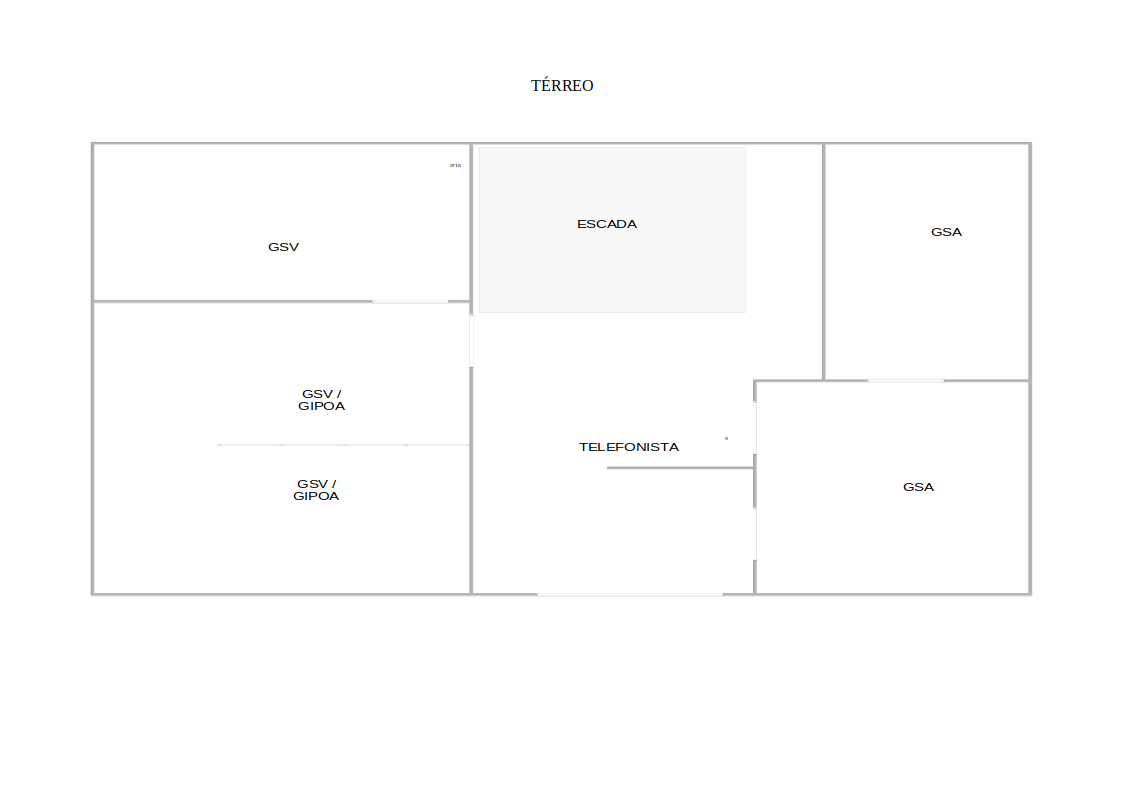
\includegraphics[height=\textwidth,width=25cm,angle=-90,keepaspectratio]{TERREO}
	\caption{SEAB/ADAPAR Térreo}
	\label{TERREO}	
\end{figure}

\begin{figure}[H]
	\centering
	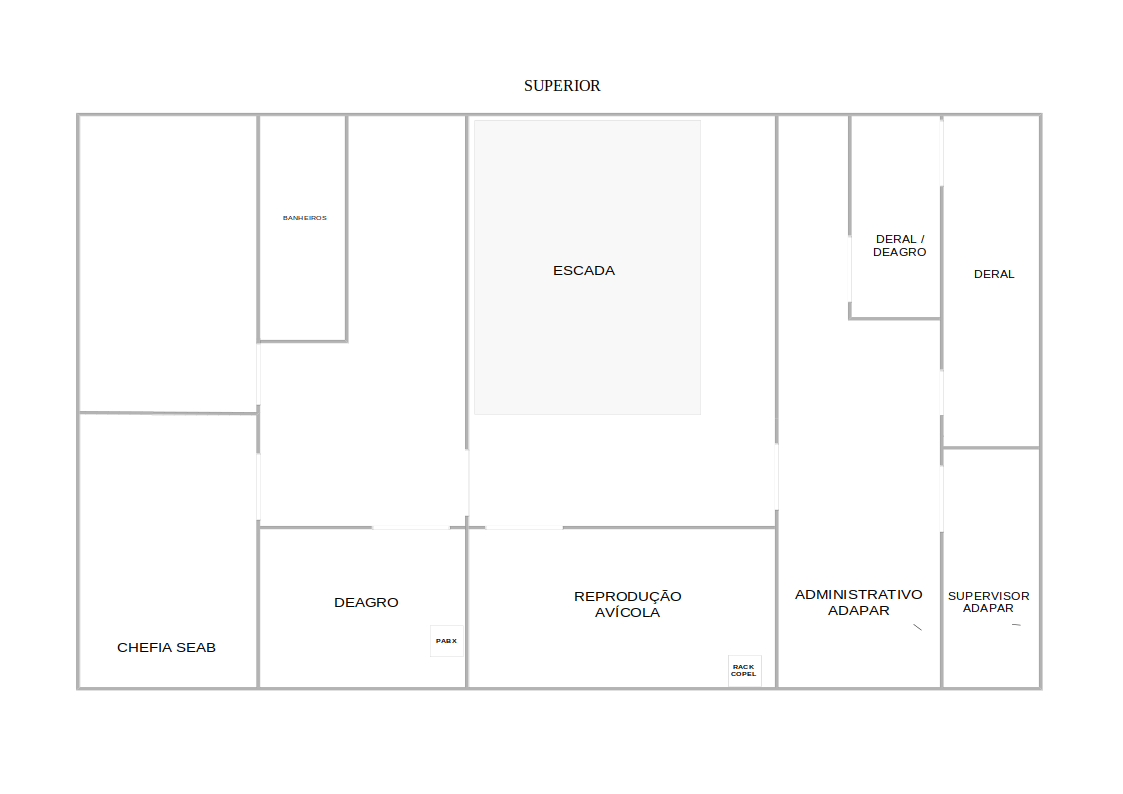
\includegraphics[height=\textwidth,width=25cm,angle=-90,keepaspectratio]{SUPERIOR}
	\caption{SEAB/ADAPAR Superior}
	\label{SUPERIOR}	
\end{figure}

\begin{figure}[H]
	\centering
	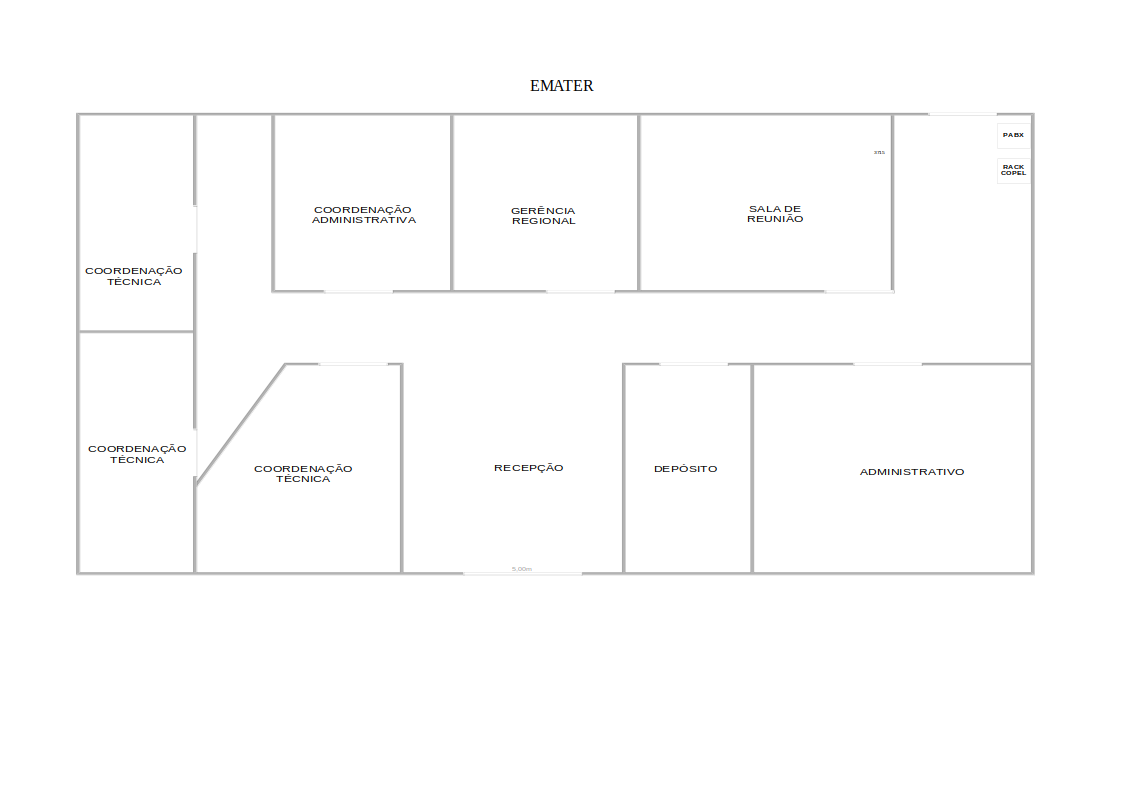
\includegraphics[height=\textwidth,width=25cm,angle=-90,keepaspectratio]{EMATER}
	\caption{EMATER}
	\label{EMATER}	
\end{figure}

\section{Planta Lógica - Elementos estruturados}

\subsection{Estado atual}
Abaixo estão as plantas atuais dos locais que serão contemplados pelo projeto: Emater (Figura \ref{EMATER ATUAL}), SEAB/ADAPAR Térro e 1º Piso (Figura \ref{SEAB/ADAPAR ATUAL}) e (Figura \ref{SEAB/ADAPAR ATUAL 1}).

\begin{figure}[H]
	\centering
	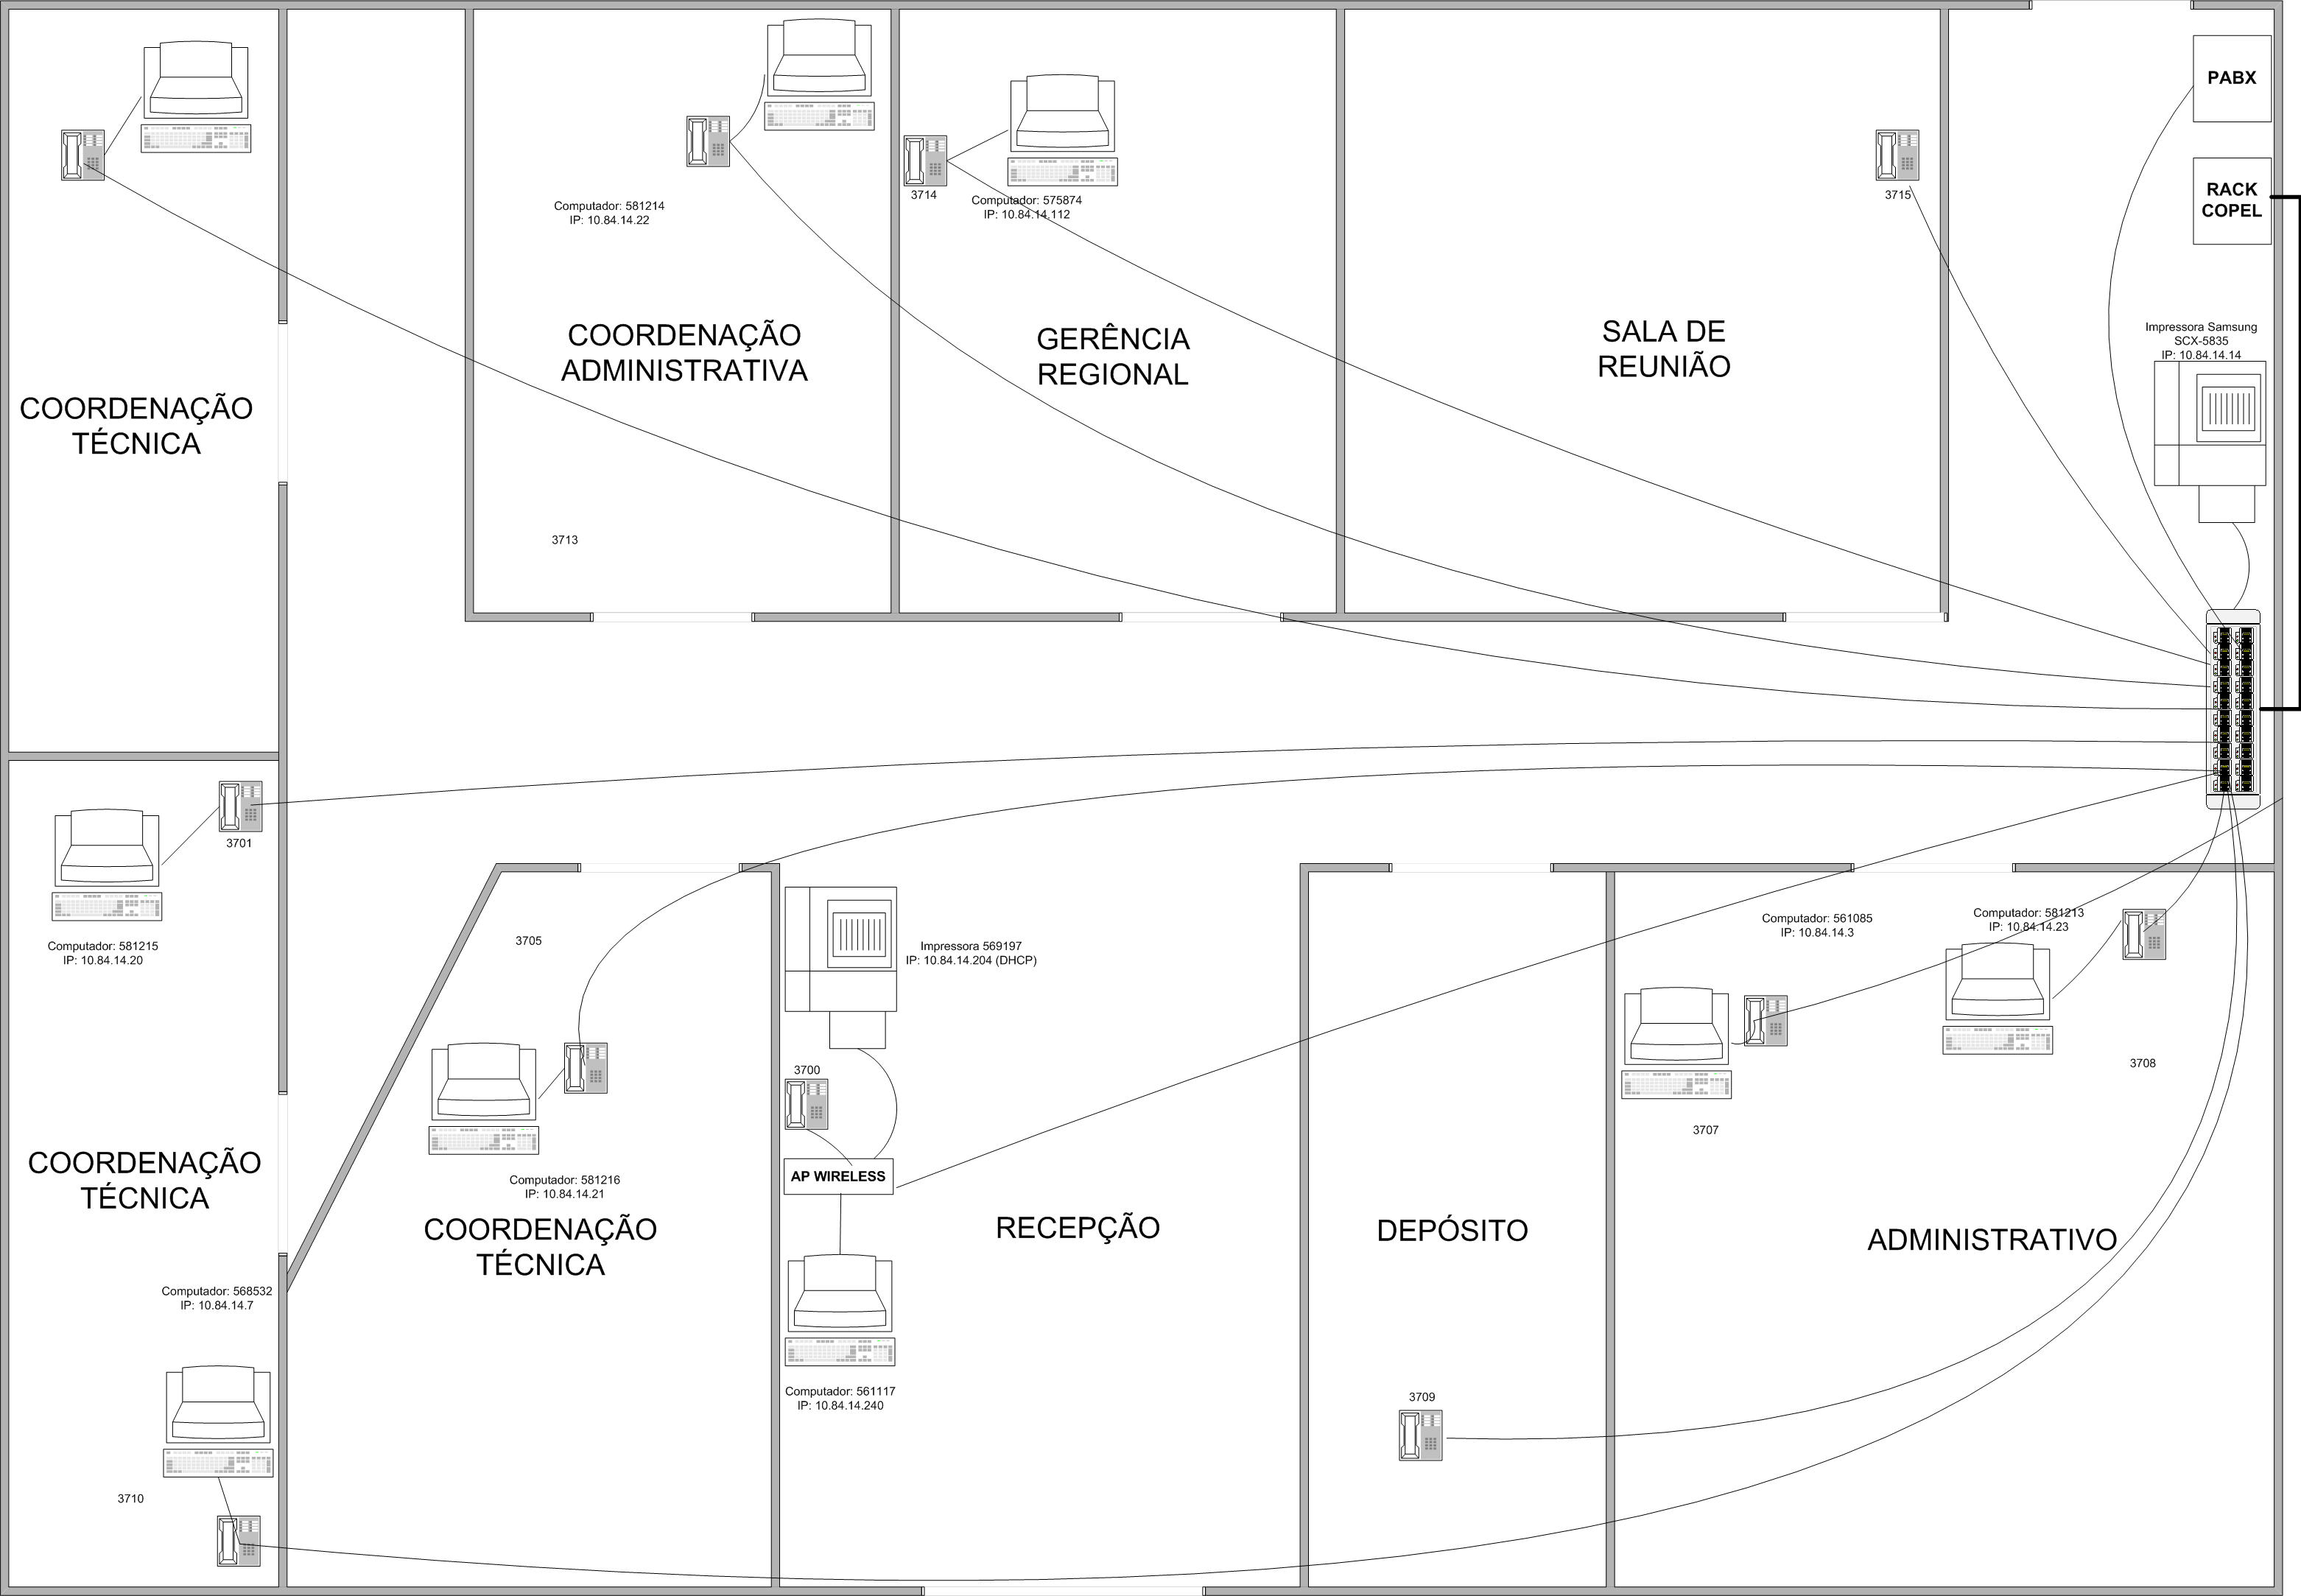
\includegraphics[height=\textwidth,width=25cm,angle=-90,keepaspectratio]{plantaemater}
	\caption{Planta atual EMATER}
	\label{EMATER ATUAL}	
\end{figure}
\begin{figure}[H]
	\centering
	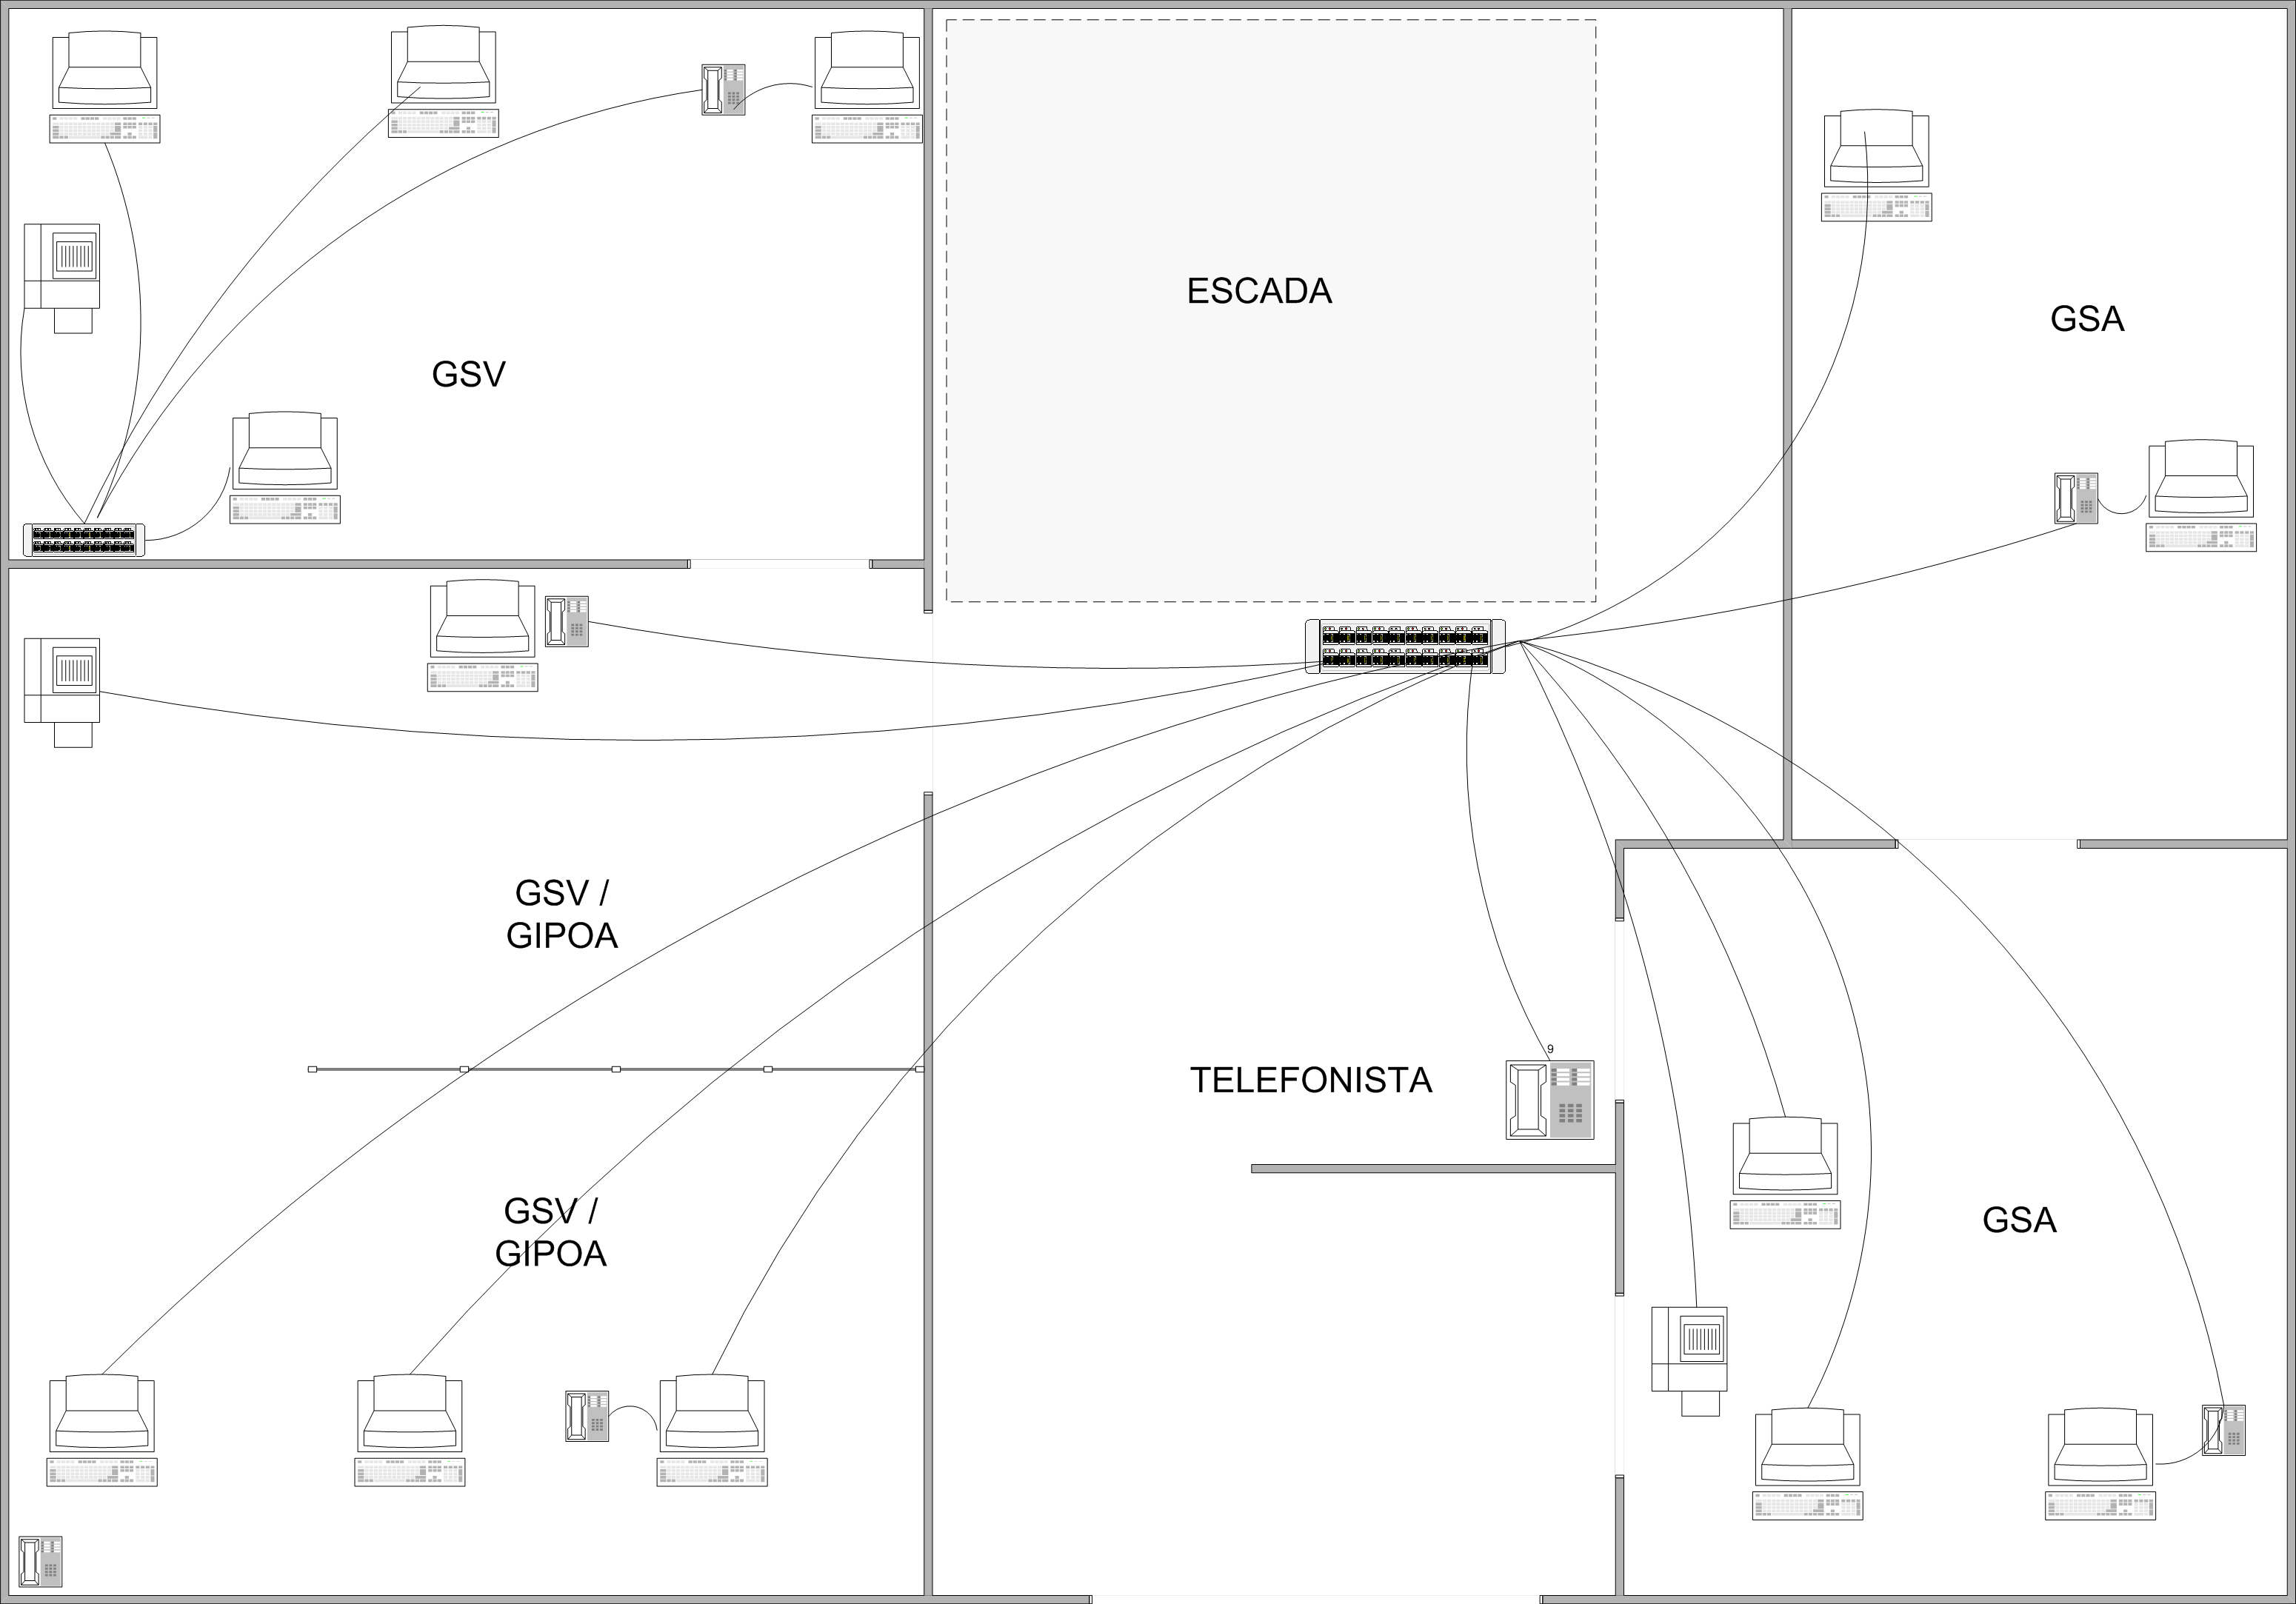
\includegraphics[height=\textwidth,width=25cm,angle=-90,keepaspectratio]{plantaseabterreo}
	\caption{Planta atual SEAB/ADAPAR  Térreo}
	\label{SEAB/ADAPAR ATUAL}	
\end{figure}
\begin{figure}[H]
	\centering
	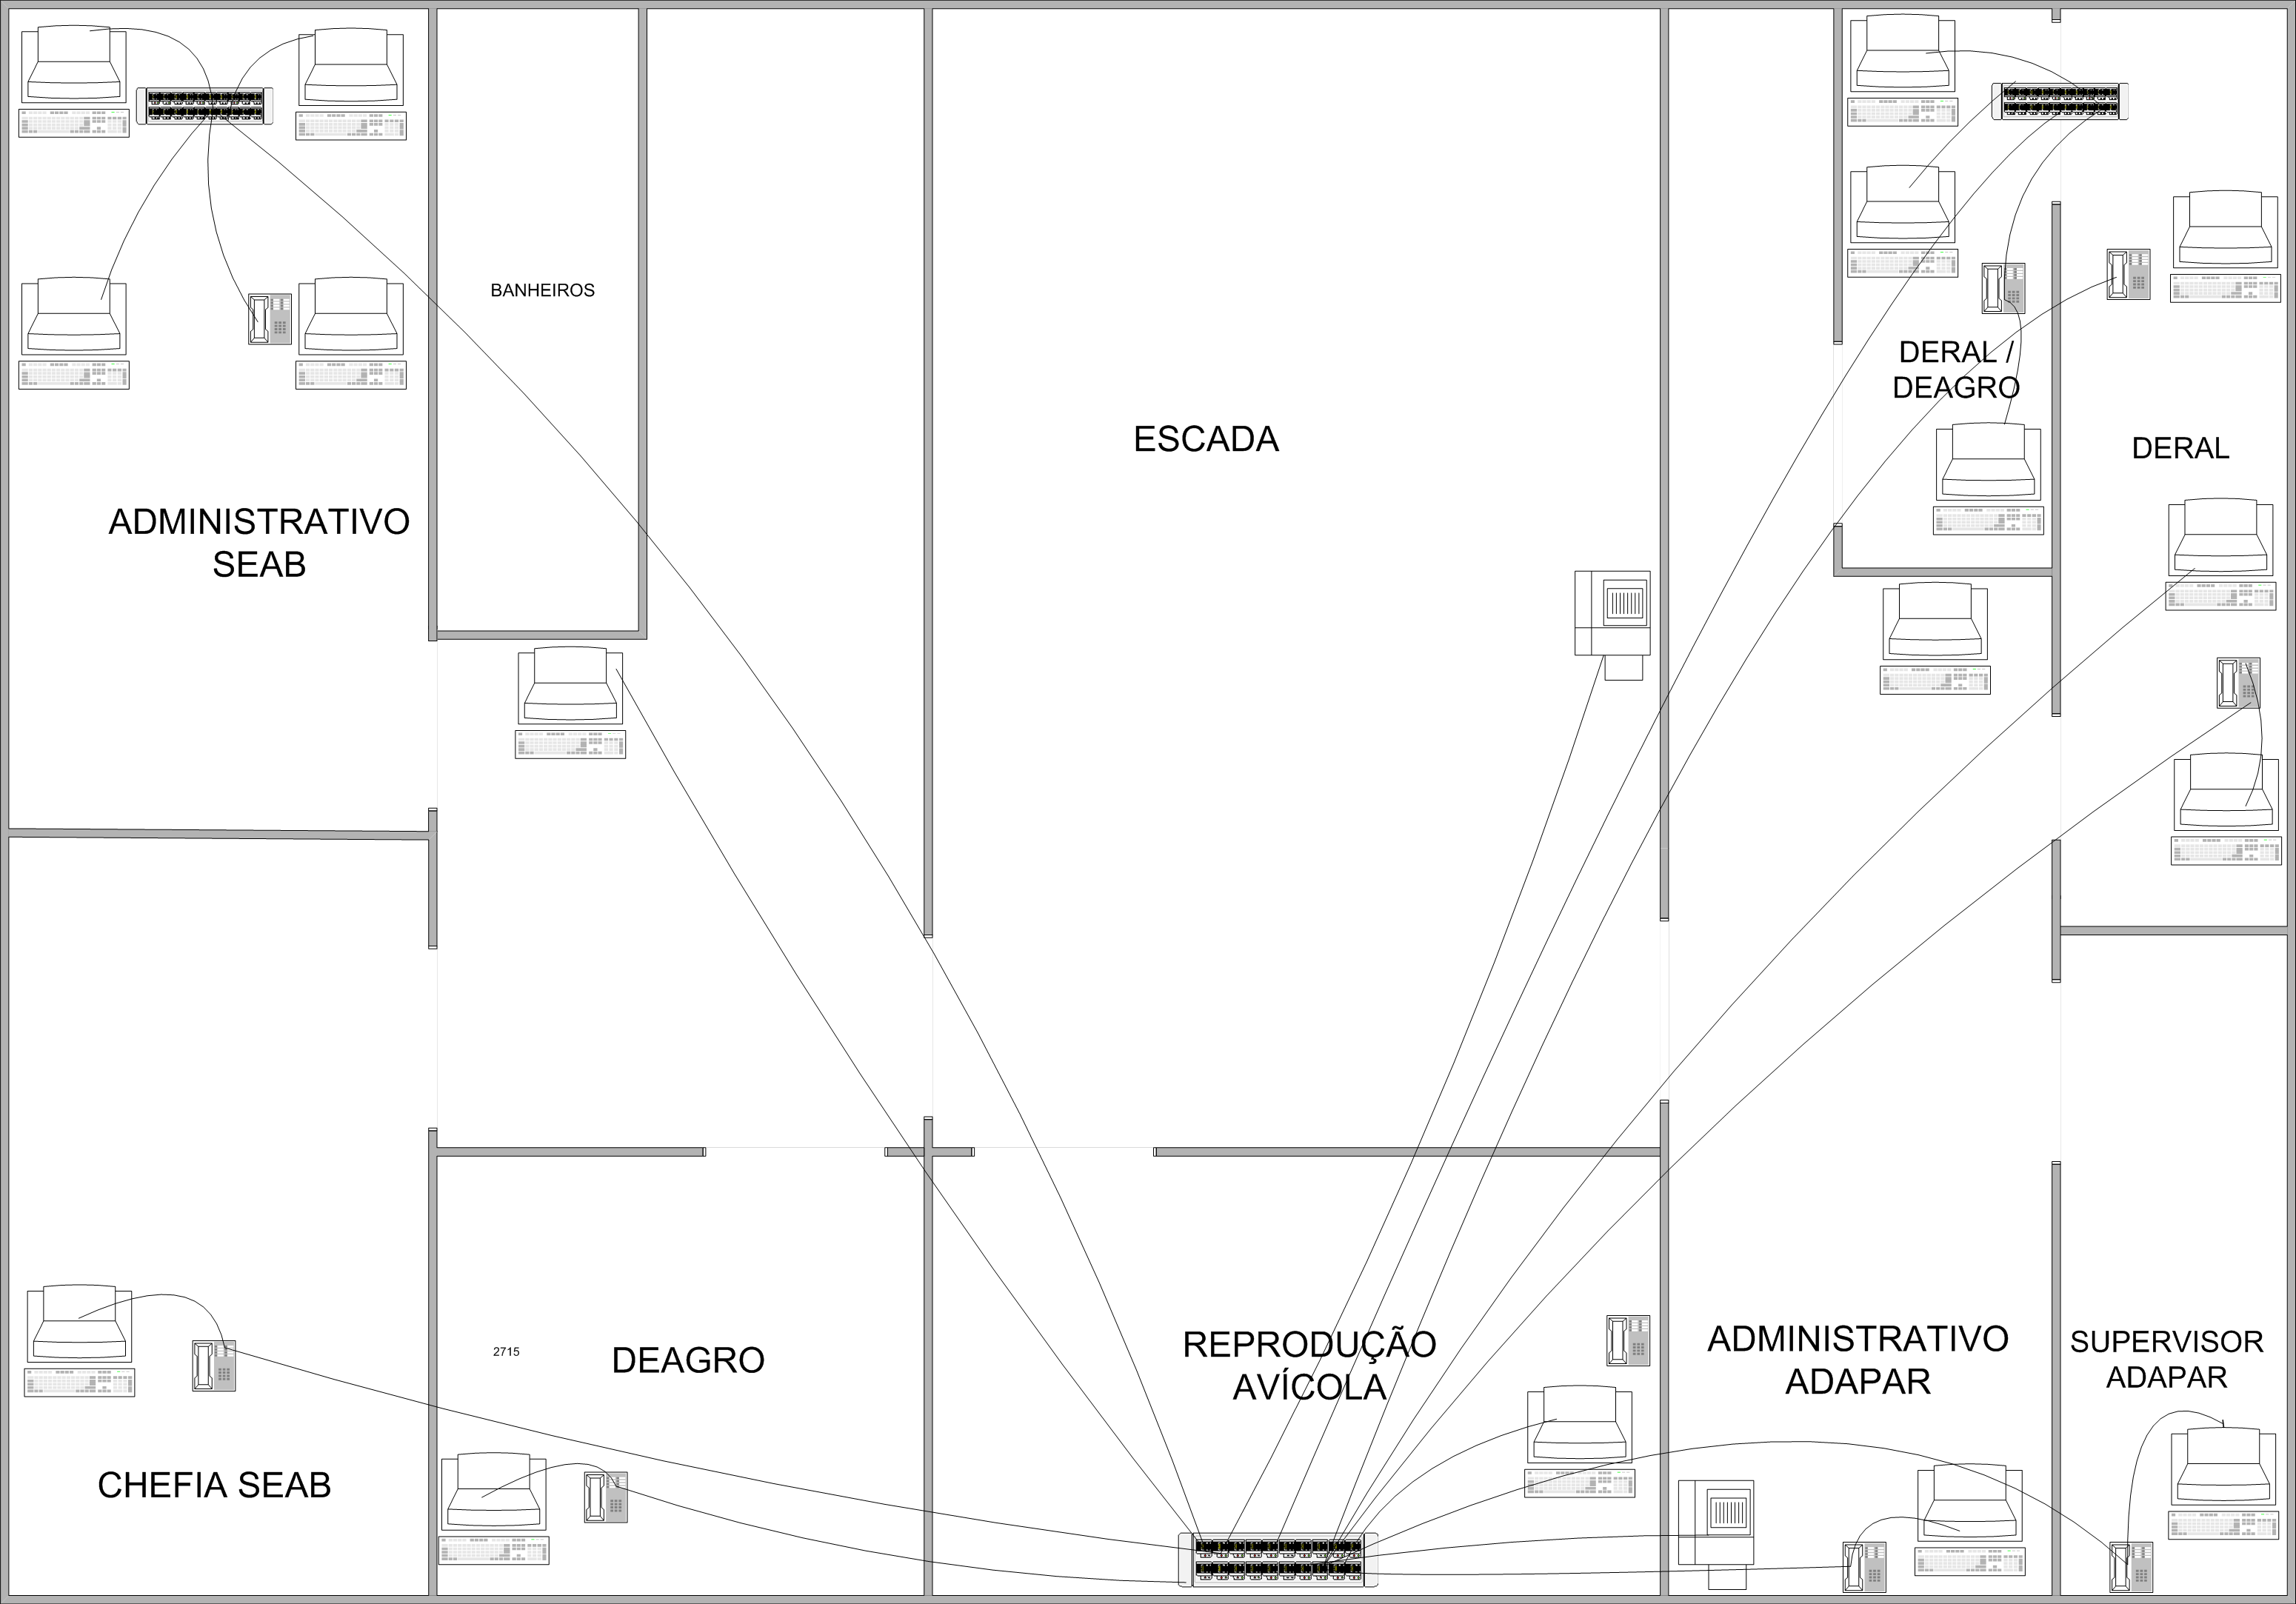
\includegraphics[height=\textwidth,width=25cm,angle=-90,keepaspectratio]{plantaseab1andar}
	\caption{Planta atual SEAB/ADAPAR Superior}
	\label{SEAB/ADAPAR ATUAL 1}	
\end{figure}

\subsection{Topologia}

Conforme levantamento de todos os dados apresentados até o momento, foi elaborada uma proposta para adequação da infraestrutura de redes dos locais. Essa proposta se baseia na aplicação de cabeamento estruturado categoria 5e para todos os passivos de redes da proposta. As imagens a seguir detalham de forma mais simples a Topologia de rede proposta (Figura \ref{TOPOLOGIA REDE}), quais serão os caminhos utilizados para lançar o cabeamento em cada um dos locais através de instalação de eletrocalhas para organização, separação e fácil identificação  (horizontal cabling) (Figura \ref{PROPOSTA EMATER}), (Figura \ref{PROPOSTA TERREO}) e (Figura \ref{PROPOSTA 1ANDAR}). Também são identificados nas imagens os pontos de rede que serão instalados por sala (work area) e identificação dos pontos próprios para a entrada no prédio do cabeamento de rede (entrance facility).

Em cada um dos 3 pisos será instalado um rack metálico fechado de 5Us que contém em cada um deles: 01 patch panel, 01 régua de tomadas elétricas, 01 switch e um organizador de cabos para patch cords conforme exemplificado na (Figura \ref{RACK}).


%Proposta futura, proposta após implantação.
%Deve conter o diagrama da rede. Atente-se a redundância  e ligações truncadas.
%Deve explicar todos termos e componentes utilizados nestas plantas. Por exemplo: entrance facility, work area, horizontal cabling, etc..

%Todos os elementos das figuras devem ser explicados. 
%Crie esboço da configuração dos racks e brackets. Explique cada um dos componentes. Você pode criar uma tabela contendo figuras dentro, ou criar uma tabela e incluí-la como imagem. Por exemplo, verifique a tabela \ref{tab1}.


\begin{figure}[H]
	\centering
	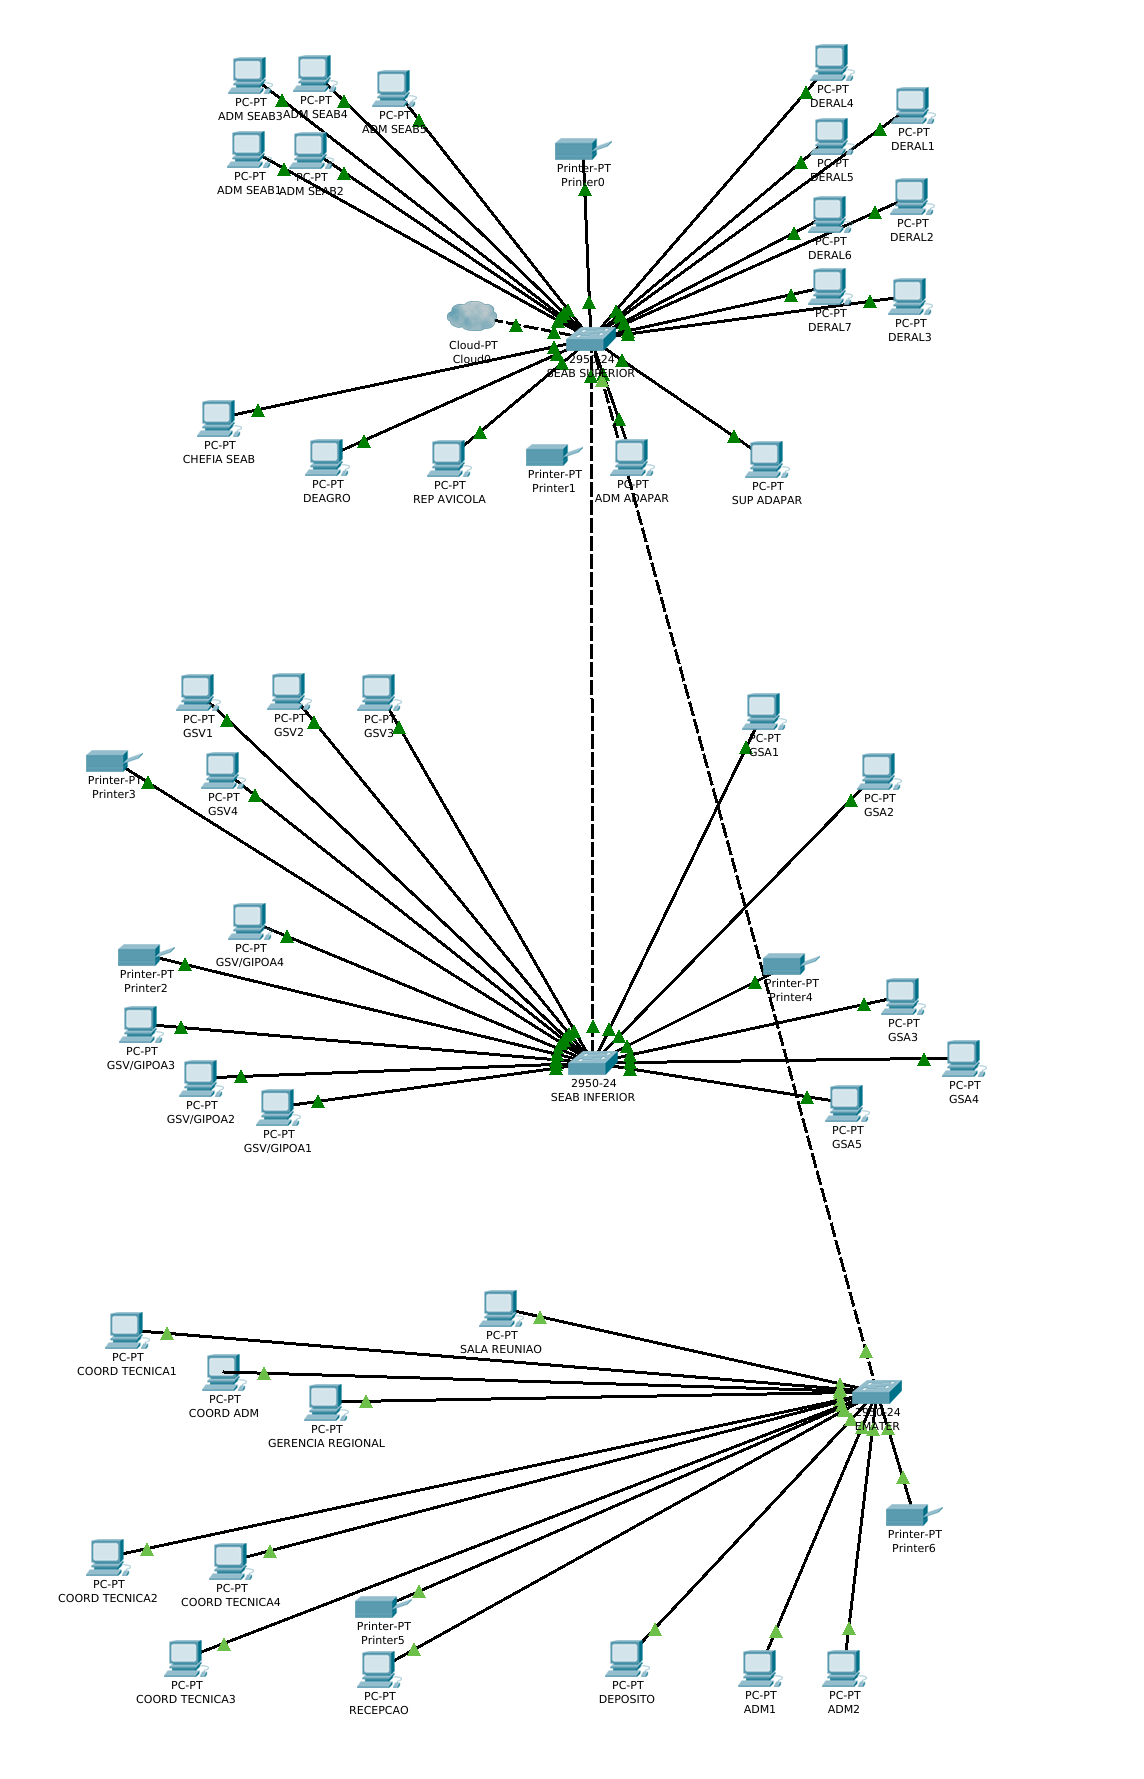
\includegraphics[height=\textwidth,width=25cm,angle=0,keepaspectratio]{topologiarede}
	\caption{Topologia da rede}
	\label{TOPOLOGIA REDE}	
\end{figure}
\begin{figure}[H]
	\centering
	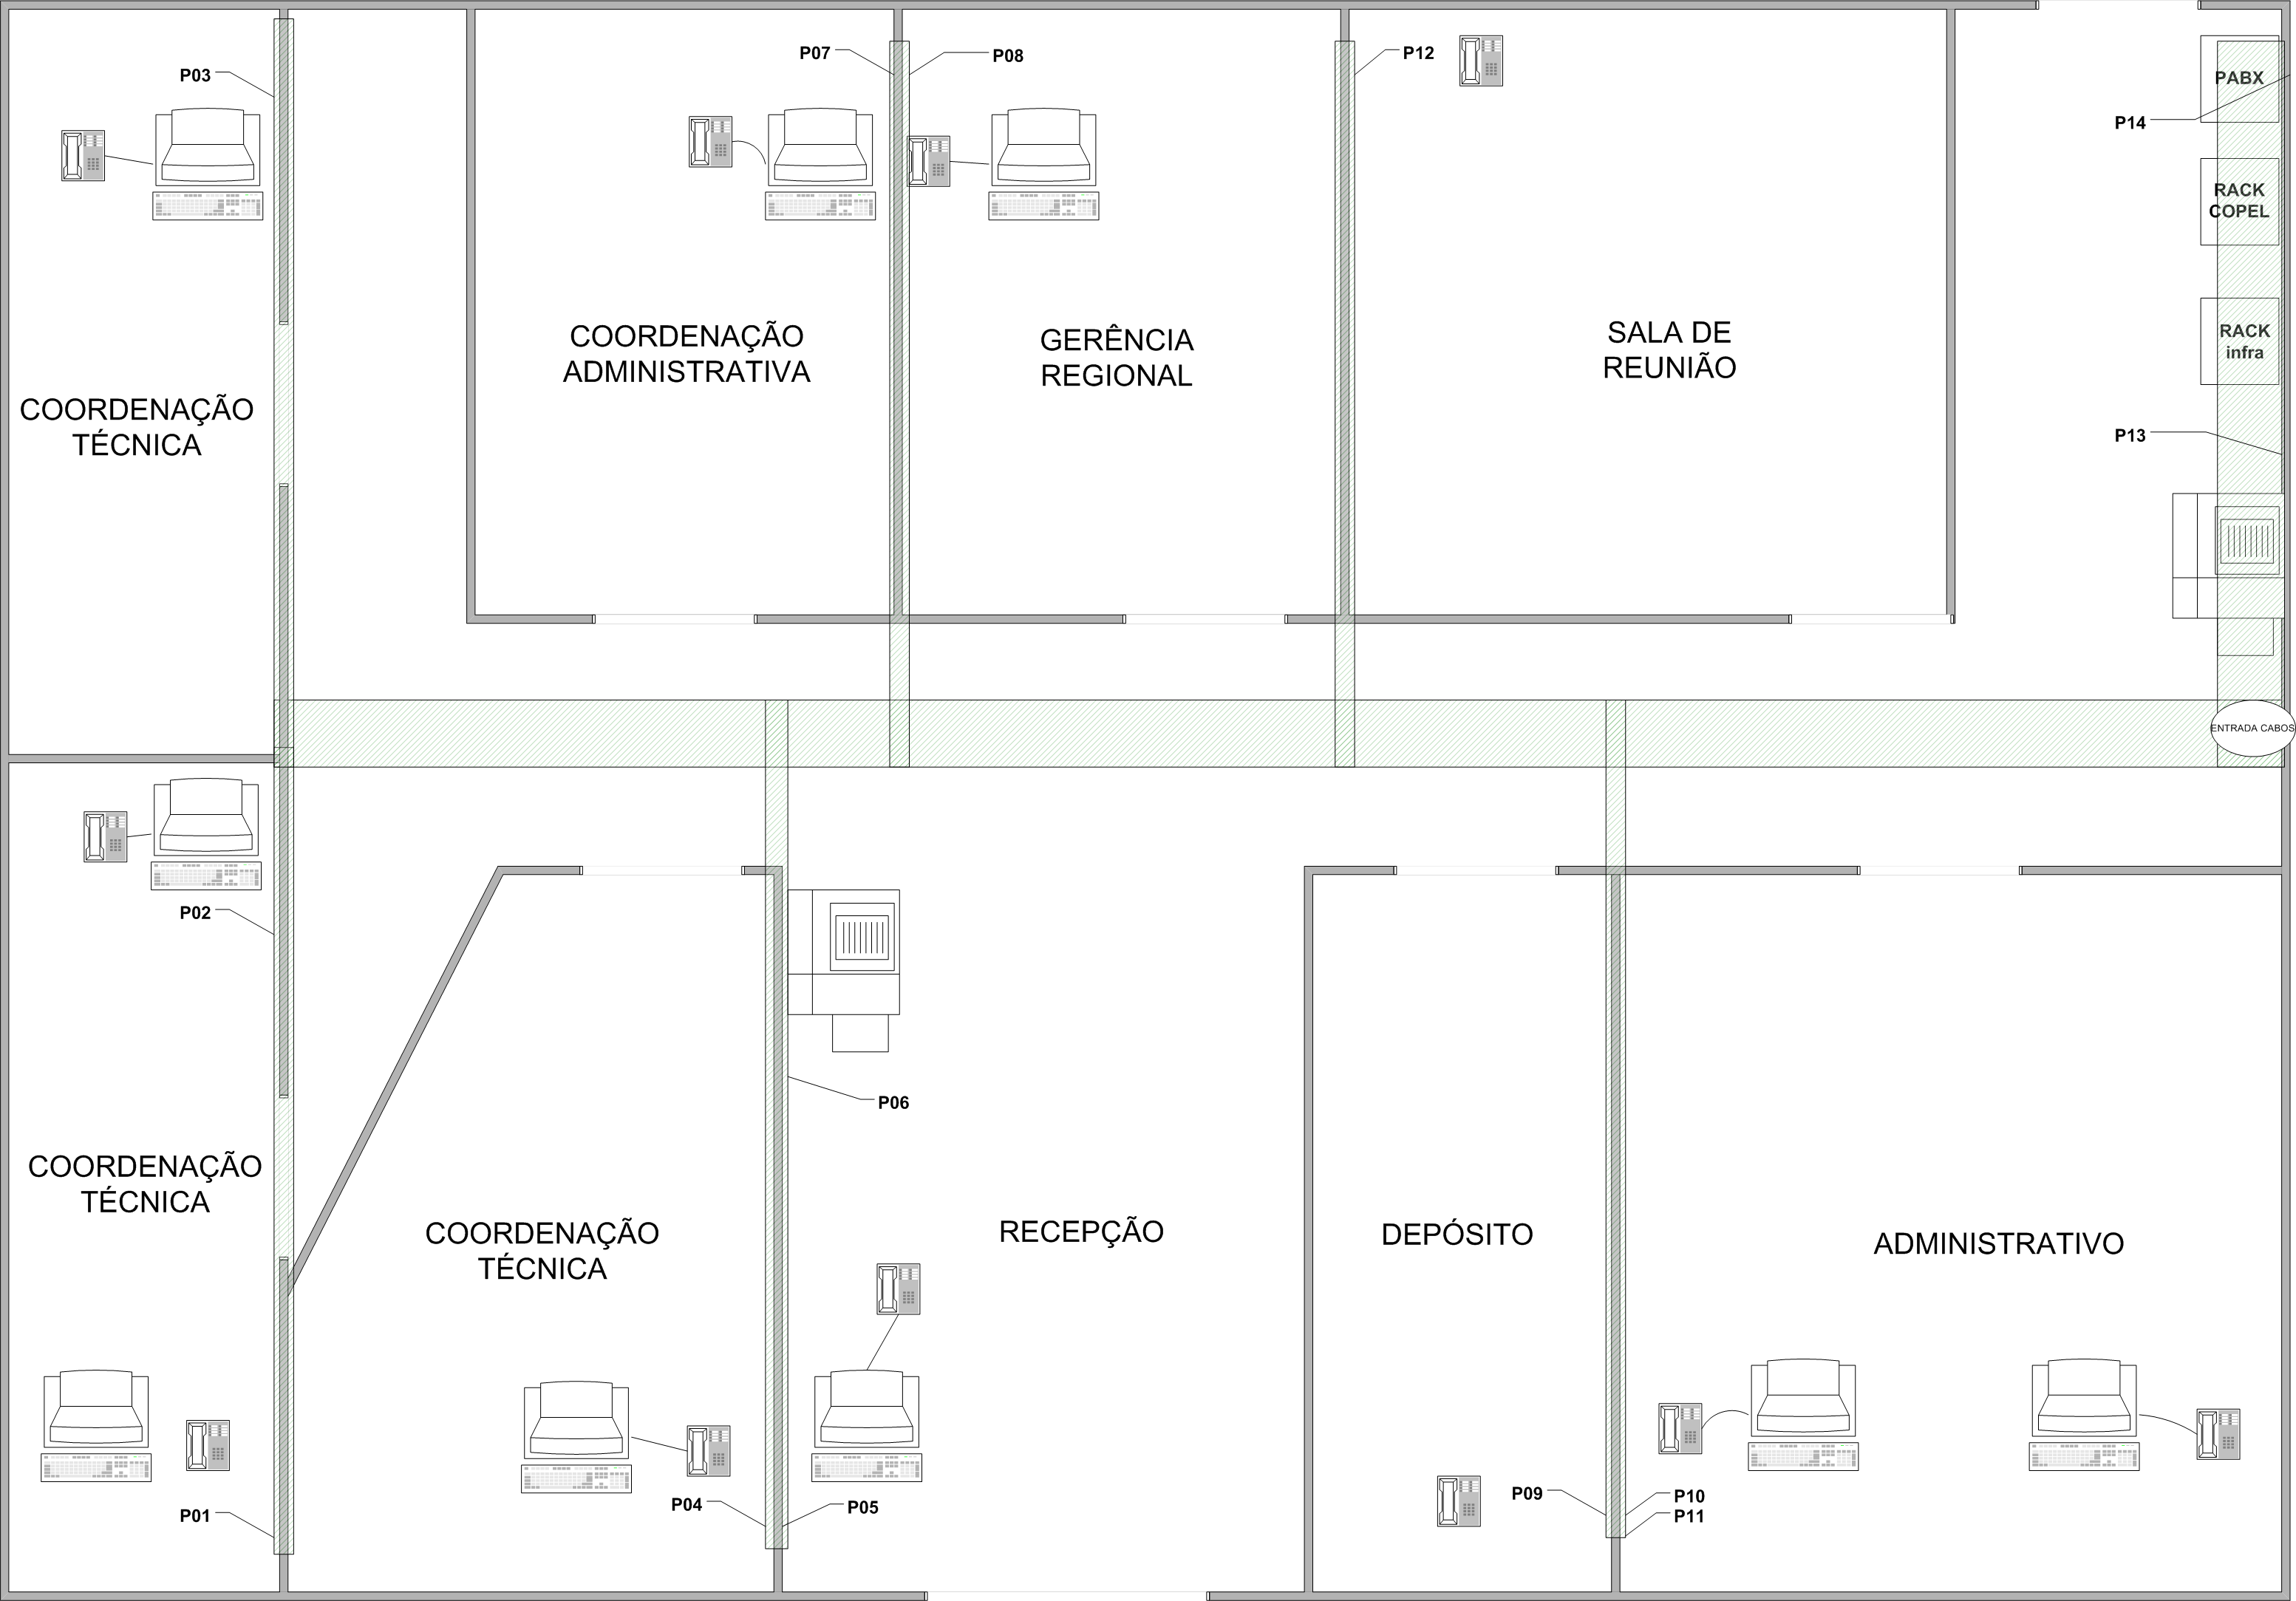
\includegraphics[height=\textwidth,width=25cm,angle=-90,keepaspectratio]{plantaematernova}
	\caption{Proposta EMATER}
	\label{PROPOSTA EMATER}	
\end{figure}
\begin{figure}[H]
	\centering
	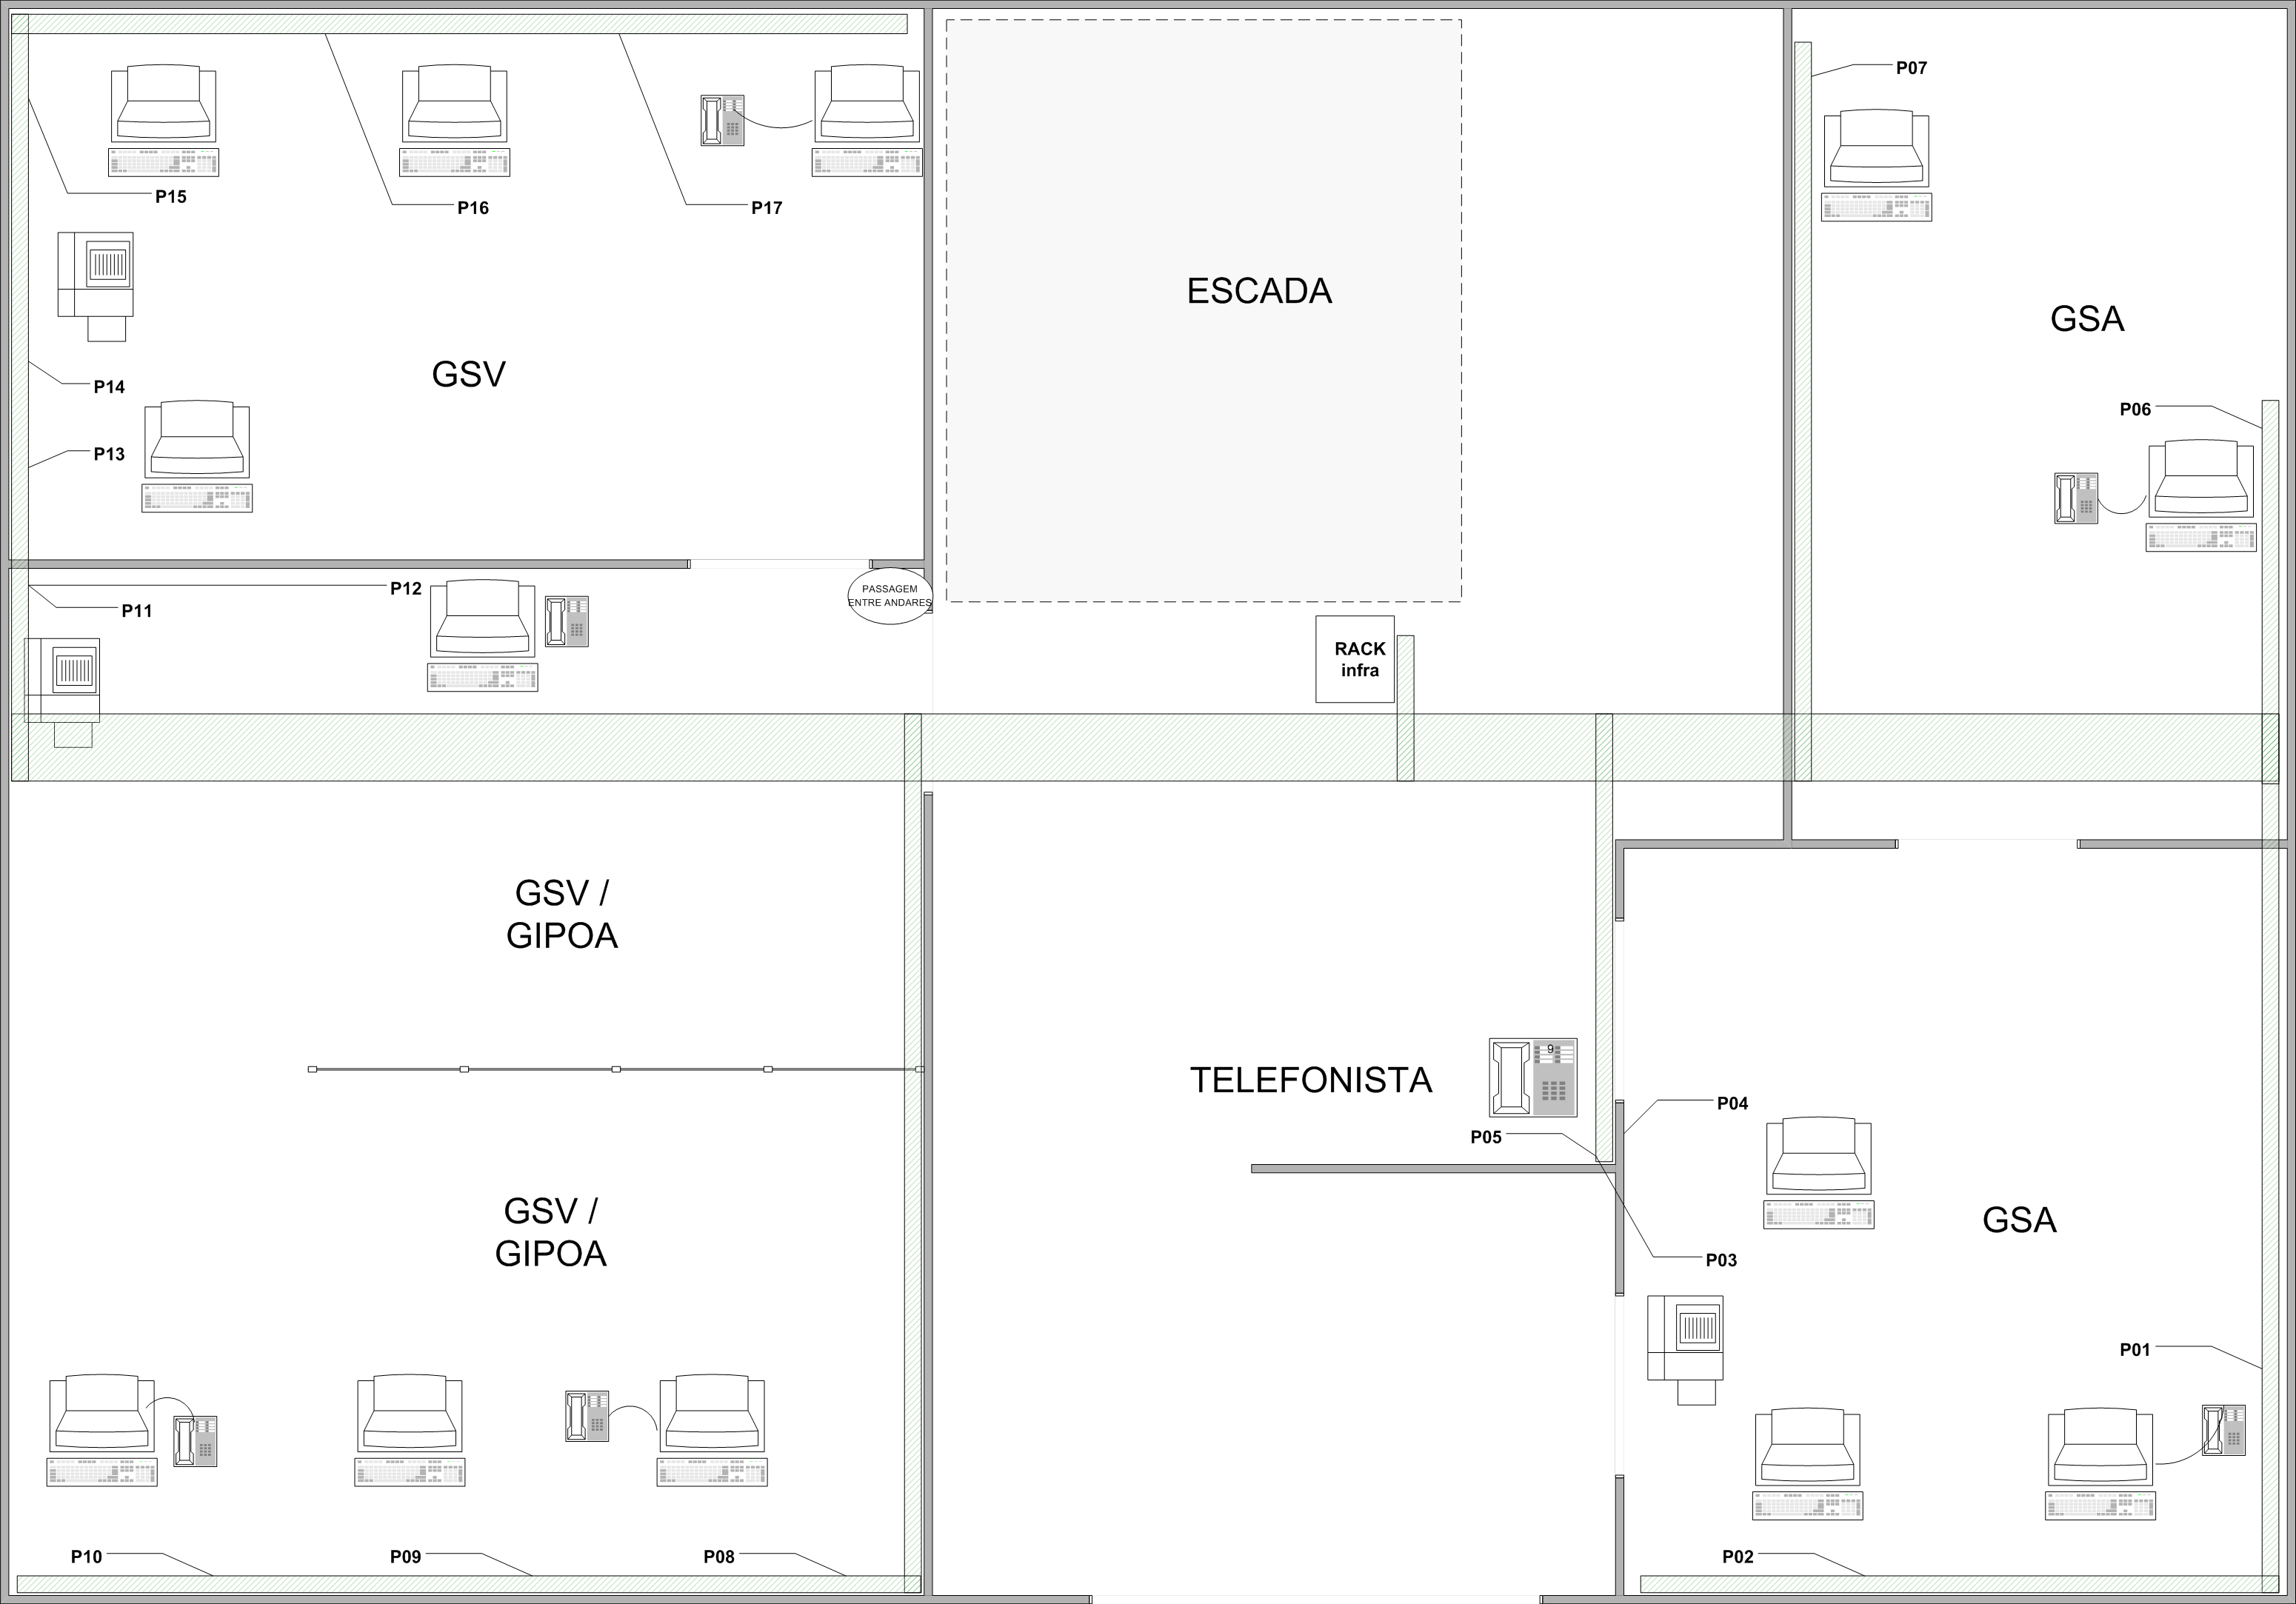
\includegraphics[height=\textwidth,width=25cm,angle=-90,keepaspectratio]{plantaseabterreonova}
	\caption{Proposta SEAB/ADAPAR Térreo}
	\label{PROPOSTA TERREO}
\end{figure}
\begin{figure}[H]
	\centering
	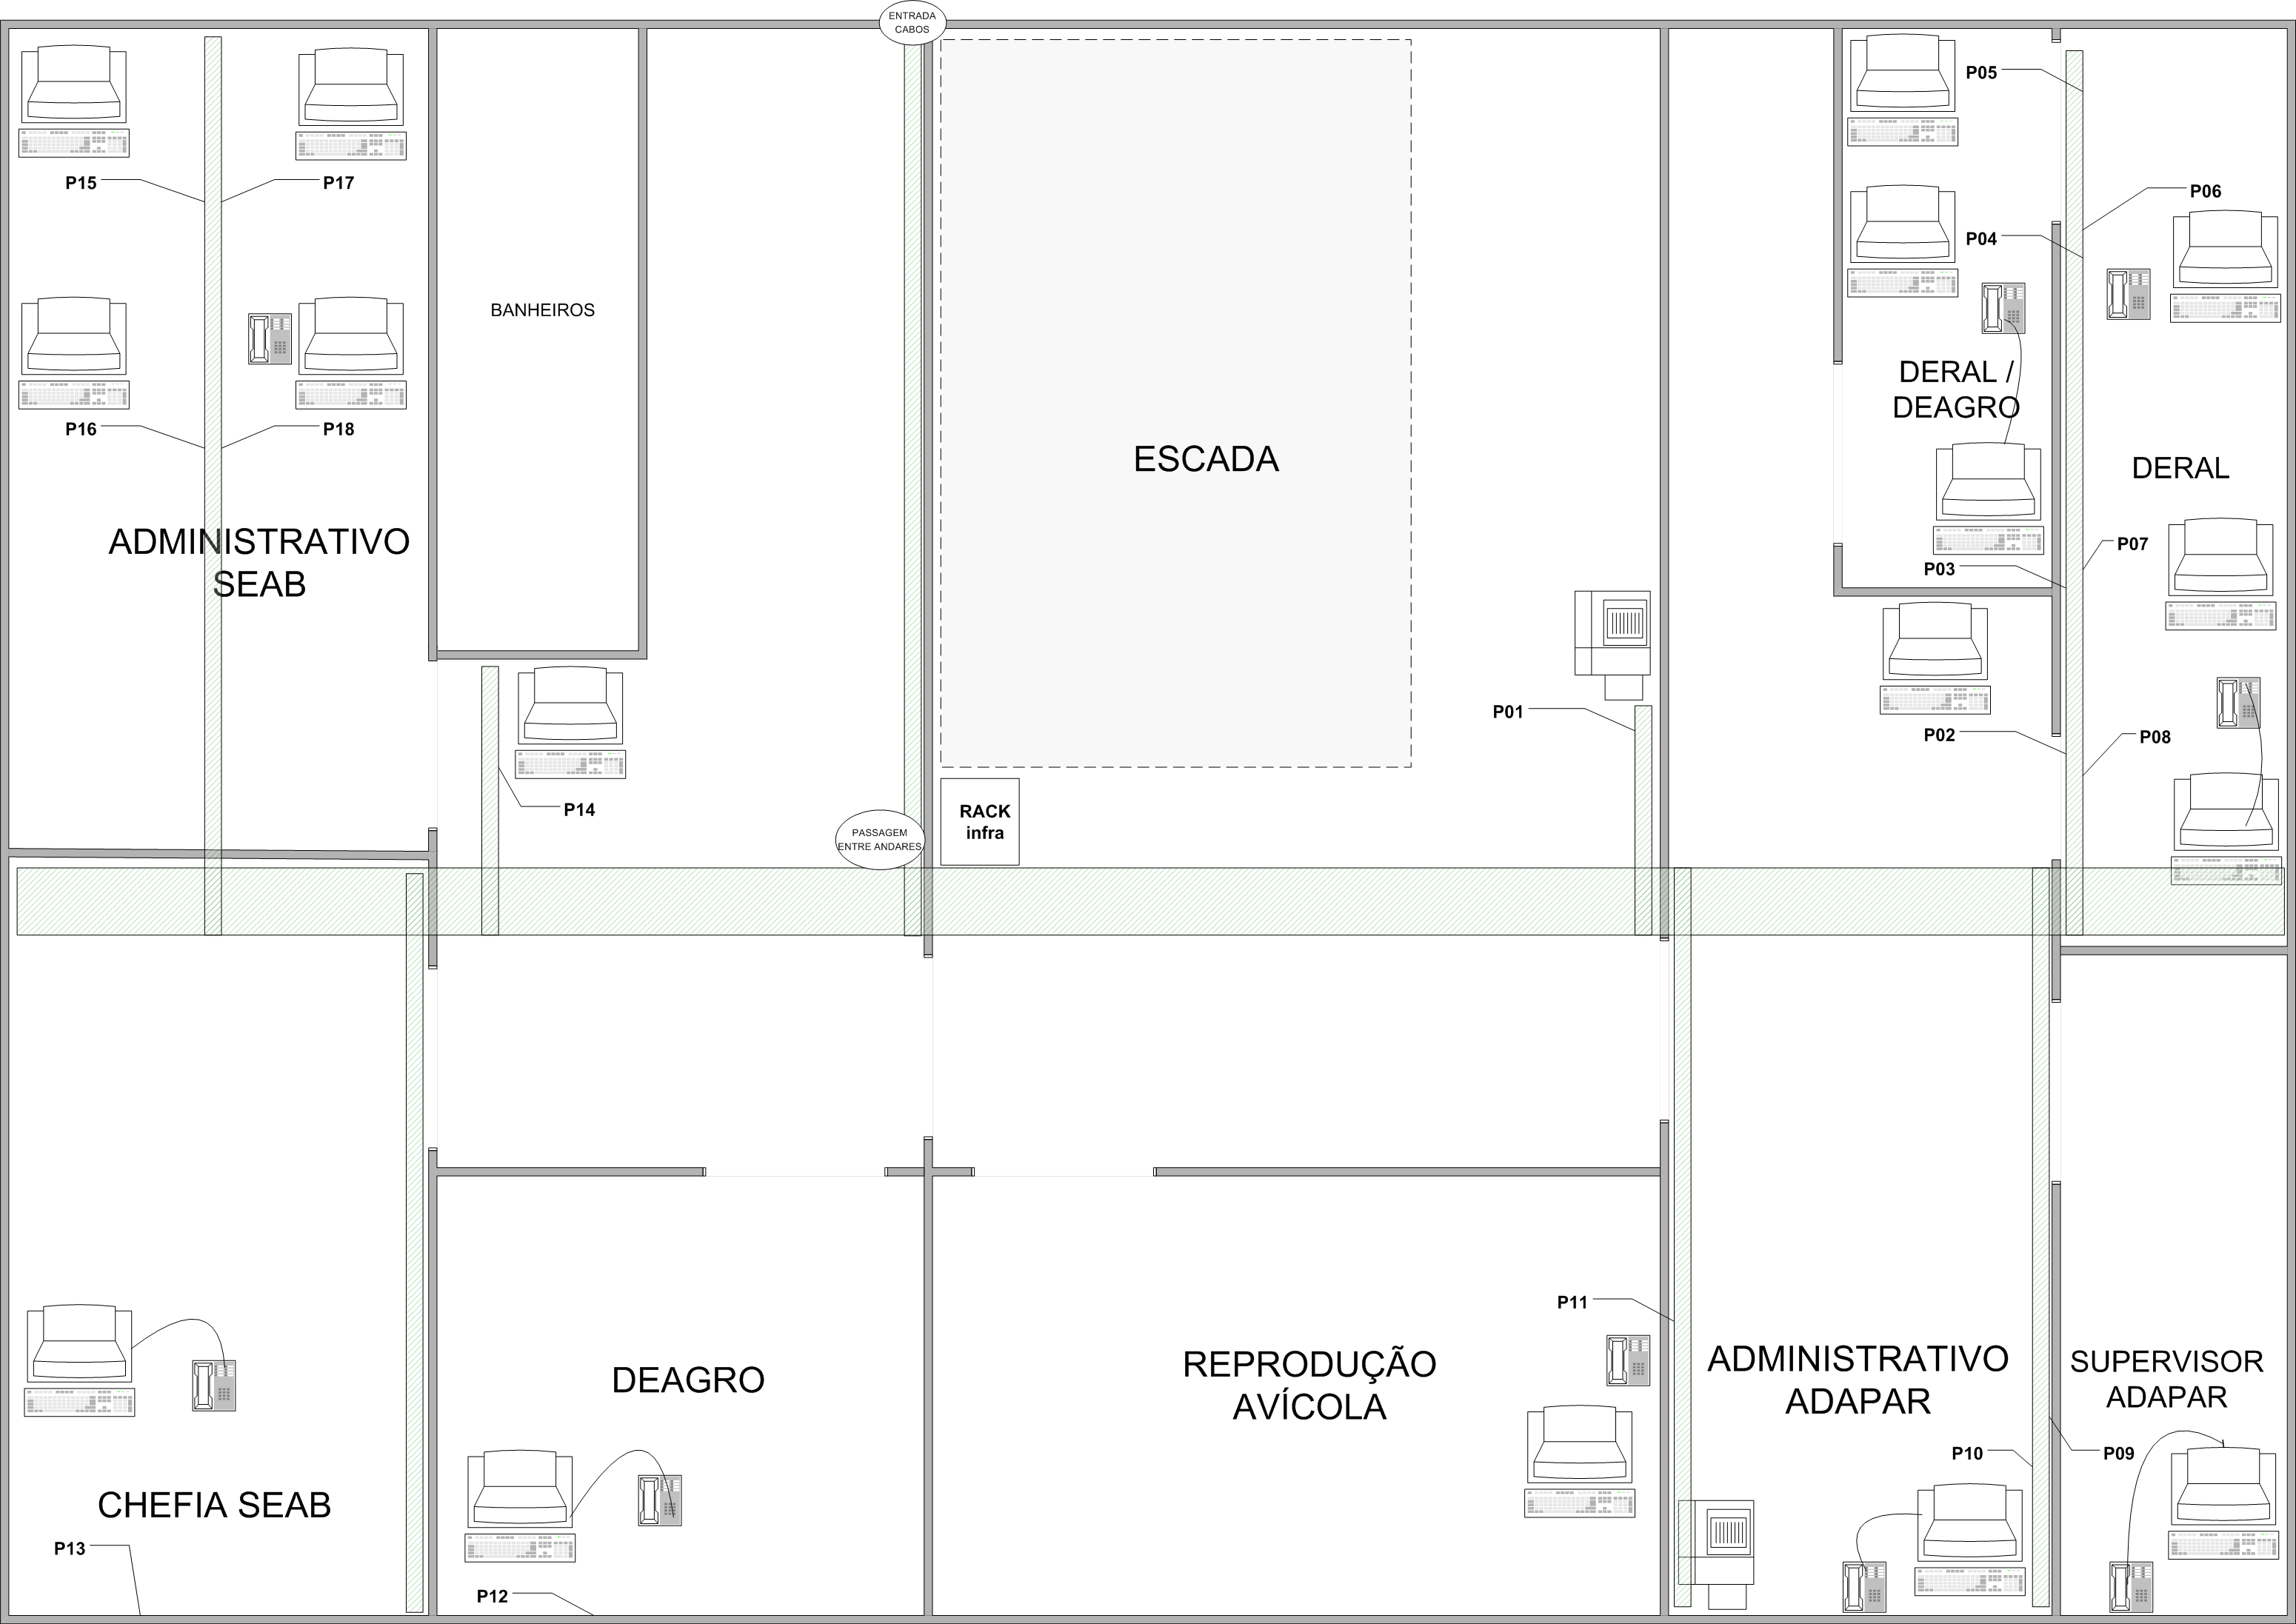
\includegraphics[height=\textwidth,width=25cm,angle=-90,keepaspectratio]{plantaseab1andarnova}
	\caption{Proposta SEAB/ADAPAR Superior}
	\label{PROPOSTA 1ANDAR}	
\end{figure}	
\begin{figure}[H]
	\centering
	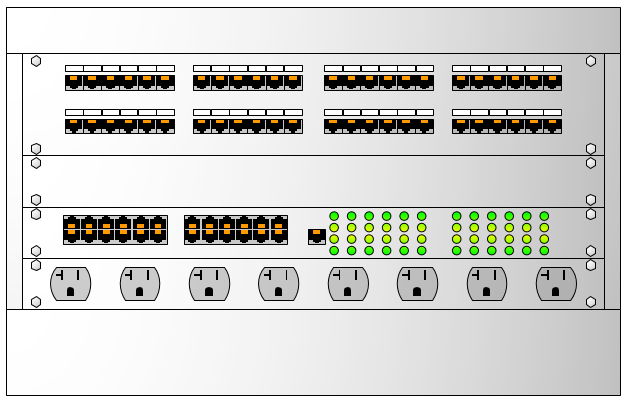
\includegraphics[height=\textwidth,width=15cm,angle=0,keepaspectratio]{rack}
	\caption{Rack 5U}
	\label{RACK}	
\end{figure}




\subsection{Encaminhamento}
O cabeamento será alojado em eletrocalhas aéreas e em calhas plásticas fixadas nas paredes.

% instaladas nos Eletrodutos, calhas, e qualquer material em que os cabos serão alojados/alocados.

\subsection{Memorial descritivo}

%Relacione todos os equipamentos passivos que serão utilizados, tipo, fabricante, quantidade.
\begin{itemize}
	\item Cabo UTP Categoria 5e; marca Furukawa; 2000 metros.
	\item Rack de parede 19” 5u; marca Protectm; 3 unidades.
	\item Patch Panel CAT 5e; marca Furukawa; 3 unidades.
	\item Organizador de cabos para rack 19"; marca PierTelecom; 3 unidades.
	\item Régua de Tomadas com padrão de fixação em rack 19"; marca IPEC; 3 unidades.
	\item Etiqueta térmica para identificação dos cabos; marca Brother; 30 metros.
	\item Patch Cords UTP CAT 5e; marca Furukawa; 90 unidades.
	\item Tomada completa externa de Telecomunicações padrão keystone com espelho; marca Pier Telecom; 45 unidades.
	\item Eletrodutos 3/4” barra de 3 metros com fixação por abraçadeira, bucha e parafuso; marca Tigre; 40 unidades;  
	\item Eletrocalha perfurada 50x100mm (larga) de 3 metros, com fixação por abraçadeira, bucha e parafuso; marca Perfil Lider, 40 unidades.
	\item Eletrocalha perfurada 50x50mm (larga) de 3 metros, com fixação por abraçadeira, bucha e parafuso; marca Perfil Lider, 32 unidades.
	\item Cabo Fibra Optica Multimodo Duplex para Uso Externo; marca MM; 70 metros.
	\item Mini DIO em aço com Pigtail; marca PierTelecom; 2 unidades.
	\item Conversor de mídia 10/100; marca TP-Link; 2 unidades.
	
\end{itemize}	

\subsection{Custos dos passivos de rede}
Abaixo estão relacionados os custos referentes aos passivos de rede necessários para a implantação do projeto conforme  Tabela \ref{custospassivos}
\begin{table}[H]
	\caption{Custos dos passivos de rede}
	\label{custospassivos} %com este label vc faz referencia no texto
	\centering
	\rotatebox{-90}{
		
	\begin{tabular}{|l|l|c|r|r|}
		\hline
		\multicolumn{1}{|c|}{Material}                                 & \multicolumn{1}{c|}{Fabricante} & Qtdade & \multicolumn{1}{c|}{Preço Un.} & \multicolumn{1}{c|}{Total} \\ \hline
		Cabo UTP Categoria 5e (metro)                                  & Furukawa                        & 2000   & R\$ 2,00                       & R\$ 4.000,00               \\ \hline
		Patch Panel CAT 5e                                             & Furukawa                        & 3      & R\$ 150,00                     & R\$ 450,00                 \\ \hline
		Rack de parede 19” 5u                                          & Protectm                        & 3      & R\$ 230,00                     & R\$ 690,00                 \\ \hline
		Tomada de Telecomunicações padrão keystone com espelho         & Pier Telecom                    & 45     & R\$ 23,50                      & R\$ 1.057,50               \\ \hline
		Régua de Tomadas com padrão de fixação em rack                 & IPEC                            & 3      & R\$ 62,00                      & R\$ 186,00                 \\ \hline
		Etiqueta de identificação dos cabos (metro)                    & Brother                         & 30     & R\$ 8,00                       & R\$ 240,00                 \\ \hline
		Patch Cords CAT 5e                                             & Furukawa                        & 90     & R\$ 12,90                      & R\$ 1.161,00               \\ \hline
		Organizador de cabos para rack                                 & Pier Telecom                    & 3      & R\$ 25,00                      & R\$ 75,00                  \\ \hline
		Eletrodutos 3/4” barra de 3 metros com fixação por abraçadeira & Tigre                           & 40     & R\$ 13,50                      & R\$ 540,00                 \\ \hline
		Eletrocalha 50x100mm 3m, c/ abraçadeira, bucha e parafuso      & Perfil Lider                    & 20     & R\$ 38,90                      & R\$ 778,00                 \\ \hline
		Eletrocalha 50x50mm 3m, c/ abraçadeira, bucha e parafuso       & Perfil Lider                    & 32     & R\$ 28,90                      & R\$ 924,80                 \\ \hline
		Cabo Fibra Optica Mult. Duplex para Uso Externo (metro)        & Info Connect                    & 70     & R\$ 4,43                       & R\$ 310,00                 \\ \hline
		Mini DIO em aço com Pigtail                                    & Pier Telecom                    & 2      & R\$ 48,00                      & R\$ 96,00                  \\ \hline
		Conversor de mídia 10/100                                      & TP-Link                         & 2      & R\$ 150,00                     & R\$ 300,00                 \\ \hline
		\textbf{TOTAL}                                                 & \multicolumn{4}{c|}{\textbf{R\$ 10.808,30}}                                                            \\ \hline
	\end{tabular}
}
\end{table}

\subsection{Identificação dos cabos}
%%Explique como os cabos serão identificados em seu projeto. Coloque uma relação dos cabos instalados e identificados.
Como serão 03 racks e 03 patch panel, os cabos serão identificados da seguinte forma: 
\begin{itemize}
\item PP01-XXX -Patch Panel 1 - Piso superior SEAB/Adapar e XXX o número do ponto na parede.
\item PP02-XXX -Patch Panel 2 - Piso térreo SEAB/Adapar e XXX o número do ponto na parede.
\item PP03-XXX -Patch Panel 3 - Emater e  XXX o número do ponto na parede.
\end{itemize}

	
\section{Implantação}
%Estabeleça um cronograma de implantação:
%Remoção de equipamentos existentes (destino para descarte), instalação dos condutores, instalação dos cabos, 
%identificação dos cabos, montagem dos racks, certificação, etc... Crie atividades e estabeleça o tempo de execução. Se for um projeto real, indique também quais os responsáveis pela execução do projeto e de cada uma das etapas.

%Defina marcas (e padrões) e fornecedores se for o caso. Atenção a contratados e subcontratados para a realização das atividades. Estabeleça a responsabilidade de execução da atividade e também da validação dela.

%Utilize algum software para gerear o cronograma. Excel,etc. O fundamental é dividir em etapas, descrever e estimar o tempo de cada uma delas.

%Segue uma relação de ferramentas:
%http://asana.com/, 
%https://trello.com/, 
%http://www.ganttproject.biz/, 
%http://www.orangescrum.org/. 
A implantação se dará na seguinte ordem:
\begin{itemize}
	\item Instalação dos racks. - 1 dia.
	\item Instalação das calhas. - 5 dias.
	\item Instalação dos eletrodutos. - 3 dias.
	\item Instalação do cabeamento. - 2 dias.
	\item Identificação dos cabos de rede conforme o padrão definido no item 6.6. - 1 dia.
	\item Montagem dos racks e os equipamentos em seu interior. - 2 dias.
	\item Certificação da rede por empresa especializada. - 1 dia.
	\item Remoção de todos o passivo de rede existente, o destino será uma empresa especializada em lixo eletônico para a correta destinação. - 1 dia.
\end{itemize}
O prazo estimado para a implantação é de 16 dias.

\section{Plano de certificação}
%Quais seriam as etapas para a certificação? 
%Quais os locais e horários para execução da certificação na rede? Toda rede será certificada?
%Como os testes seriam executados?
%Quais relatórios de certificação serão (ou deveriam ser) entregues? 
A certificação do cabeamento se dará por empresa terceirizada especializada.
A certificação será feita antes da liberação da rede para uso.
A rede será certificada por etapas, primeiro o piso superior da SEAB/ADAPAR, depois o piso térreo da SEAB/ADAPAR e por último o prédio da EMATER, resultando em uma rede totalmente certificada. 
Os testes deverão ser executados com certificador que atenda as normas vigentes. Os relatórios de certificação deverão ser entregues no prazo máximo de uma semana após a certificação dos cabos.

%\section{Plano de manutenção}

%Revisões periódicas na rede, emissão de certificados para novos pontos.

%\subsection{Plano de expansão}
%Existe um plano de expansão? Quantos novos pontos poderão ser acrecidos na rede, antes de migração de equipamentos na camada 2? Se houver expansão, quais equipamentos deverão ser direcionados para as estremidades da rede? 

%\section{Risco}
%Enumerar e explicar os riscos do projeto.

%\section{Orçamento}
%Crie uma relação de orçamentos baseado na seções anteriores.

%\section{Recomendações}
%Observações e recomendações para o cliente.

%\section{Referências bibliográficas}
%Utilize o mendley, o jabref ou diretamente o bibtex para gerenciar suas referências biliográficas. As referências são criadas automaticamente de acordo com o uso no texto.

%Exemplo: Redes de computadores, segundo \cite{t2013} é considerada..... Já \cite{kurose2010} apresenta uma versão...

%Analisando os pressupostos de \cite{ref3} e \cite{ref4} concluimos que....


%\renewcommand\refname{} %%Referências bibliográficas}  
%\bibliographystyle{ieeetr}
%\bibliography{referencias}  

%% ***********************************************************************
%% === remover daqui =====================================================
%% ***********************************************************************
%=================================================
%\section{Elementos textuais - Alguns exemplos}

%Esta seção apresenta exemplos de elementos textuais. \textbf{Remova-a da versão final do texto}.


%\subsection{Colocar elementos em itens}

%Texto antes da lista

%\begin{itemize}
%	\item First item in a list 
%	\item Second item in a list 
%	\item Third item in a list
%\end{itemize}

%\subsubsection{Uma subseção de terceiro nivel}

%Exemplo de uma subseção

%\subsection{Tabelas}

%Utilize o site http://www.tablesgenerator.com/ para elaborar as tabelas de seu trabalho.
%Para adicionar uma tabela utilize: a tag input, passando o arquivo da tabela como parametro

%\begin{table}[h!] % coloque h! para forcar a posicao
\centering
\caption{Modifique a legenda e crie um label}
\label{tab2} %com este label vc faz referencia no texto
\begin{tabular}{|l|l|l|l|l|}
\hline
\multicolumn{1}{|c|}{\textbf{Este é um exemplo de tabela}} & \multicolumn{2}{c|}{\textbf{C1}} & \multicolumn{2}{c|}{\textbf{C2}} \\ \hline
Você pode criar a tabela no excel                          & 1              & 2               & 3               & 4              \\ \hline
Exportar para CSV                                          & 5              & 6               & 7               & 8              \\ \hline
E importar no Table Generator                              & 9              & 10              &                 &                \\ \hline
\multicolumn{5}{|c|}{\textit{Gere o tex, e adicione em seu arquivo}}                                                             \\ \hline
\end{tabular}
\end{table}

%Dentro do arquivo você deve definir o label e pode utilizá-lo para referenciar. Exemplo:
%Na tab \ref{tab2} temos a relação de ....


%Você também pode modificar a tabela manualmente, incluindo, por exemplo h! dentro de sua definição. Veja no exemplo tab2.tex

%\subsection{Figuras}

%As figuras podem ser no formato PDF, JPG, PNG. Você pode referenciá-las da mesma maneira que tabelas. Exemplo: A figura \ref{fig1} apresenta.....

%Não se preocupe o local em que a figura será renderizada em seu texto. Preocupe-se em criar referência para ela, ou seja, toda figura e tabela deve conter pelo menos uma referência no texto.

%\begin{figure}
%\centering
%\includegraphics[width=\textwidth]{fig1}
%\caption{Exemplo de figura com escala horizontal}
%\label{fig1}
%\end{figure}


%\begin{figure}
%	\centering
%	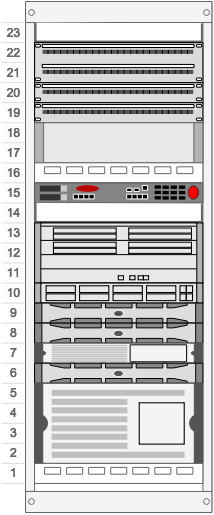
\includegraphics[]{fig2}
%	\caption{Exemplo de figura sem escala}
%	\label{fig2}
%\end{figure}

%Você pode rotacionar figuras também. Para isso utilize o parâmetro angle=-90. Repare que a escala da figura foi modificada pelo parametro height. Você também pode utilizar scale

%\begin{figure}
%	\centering
%	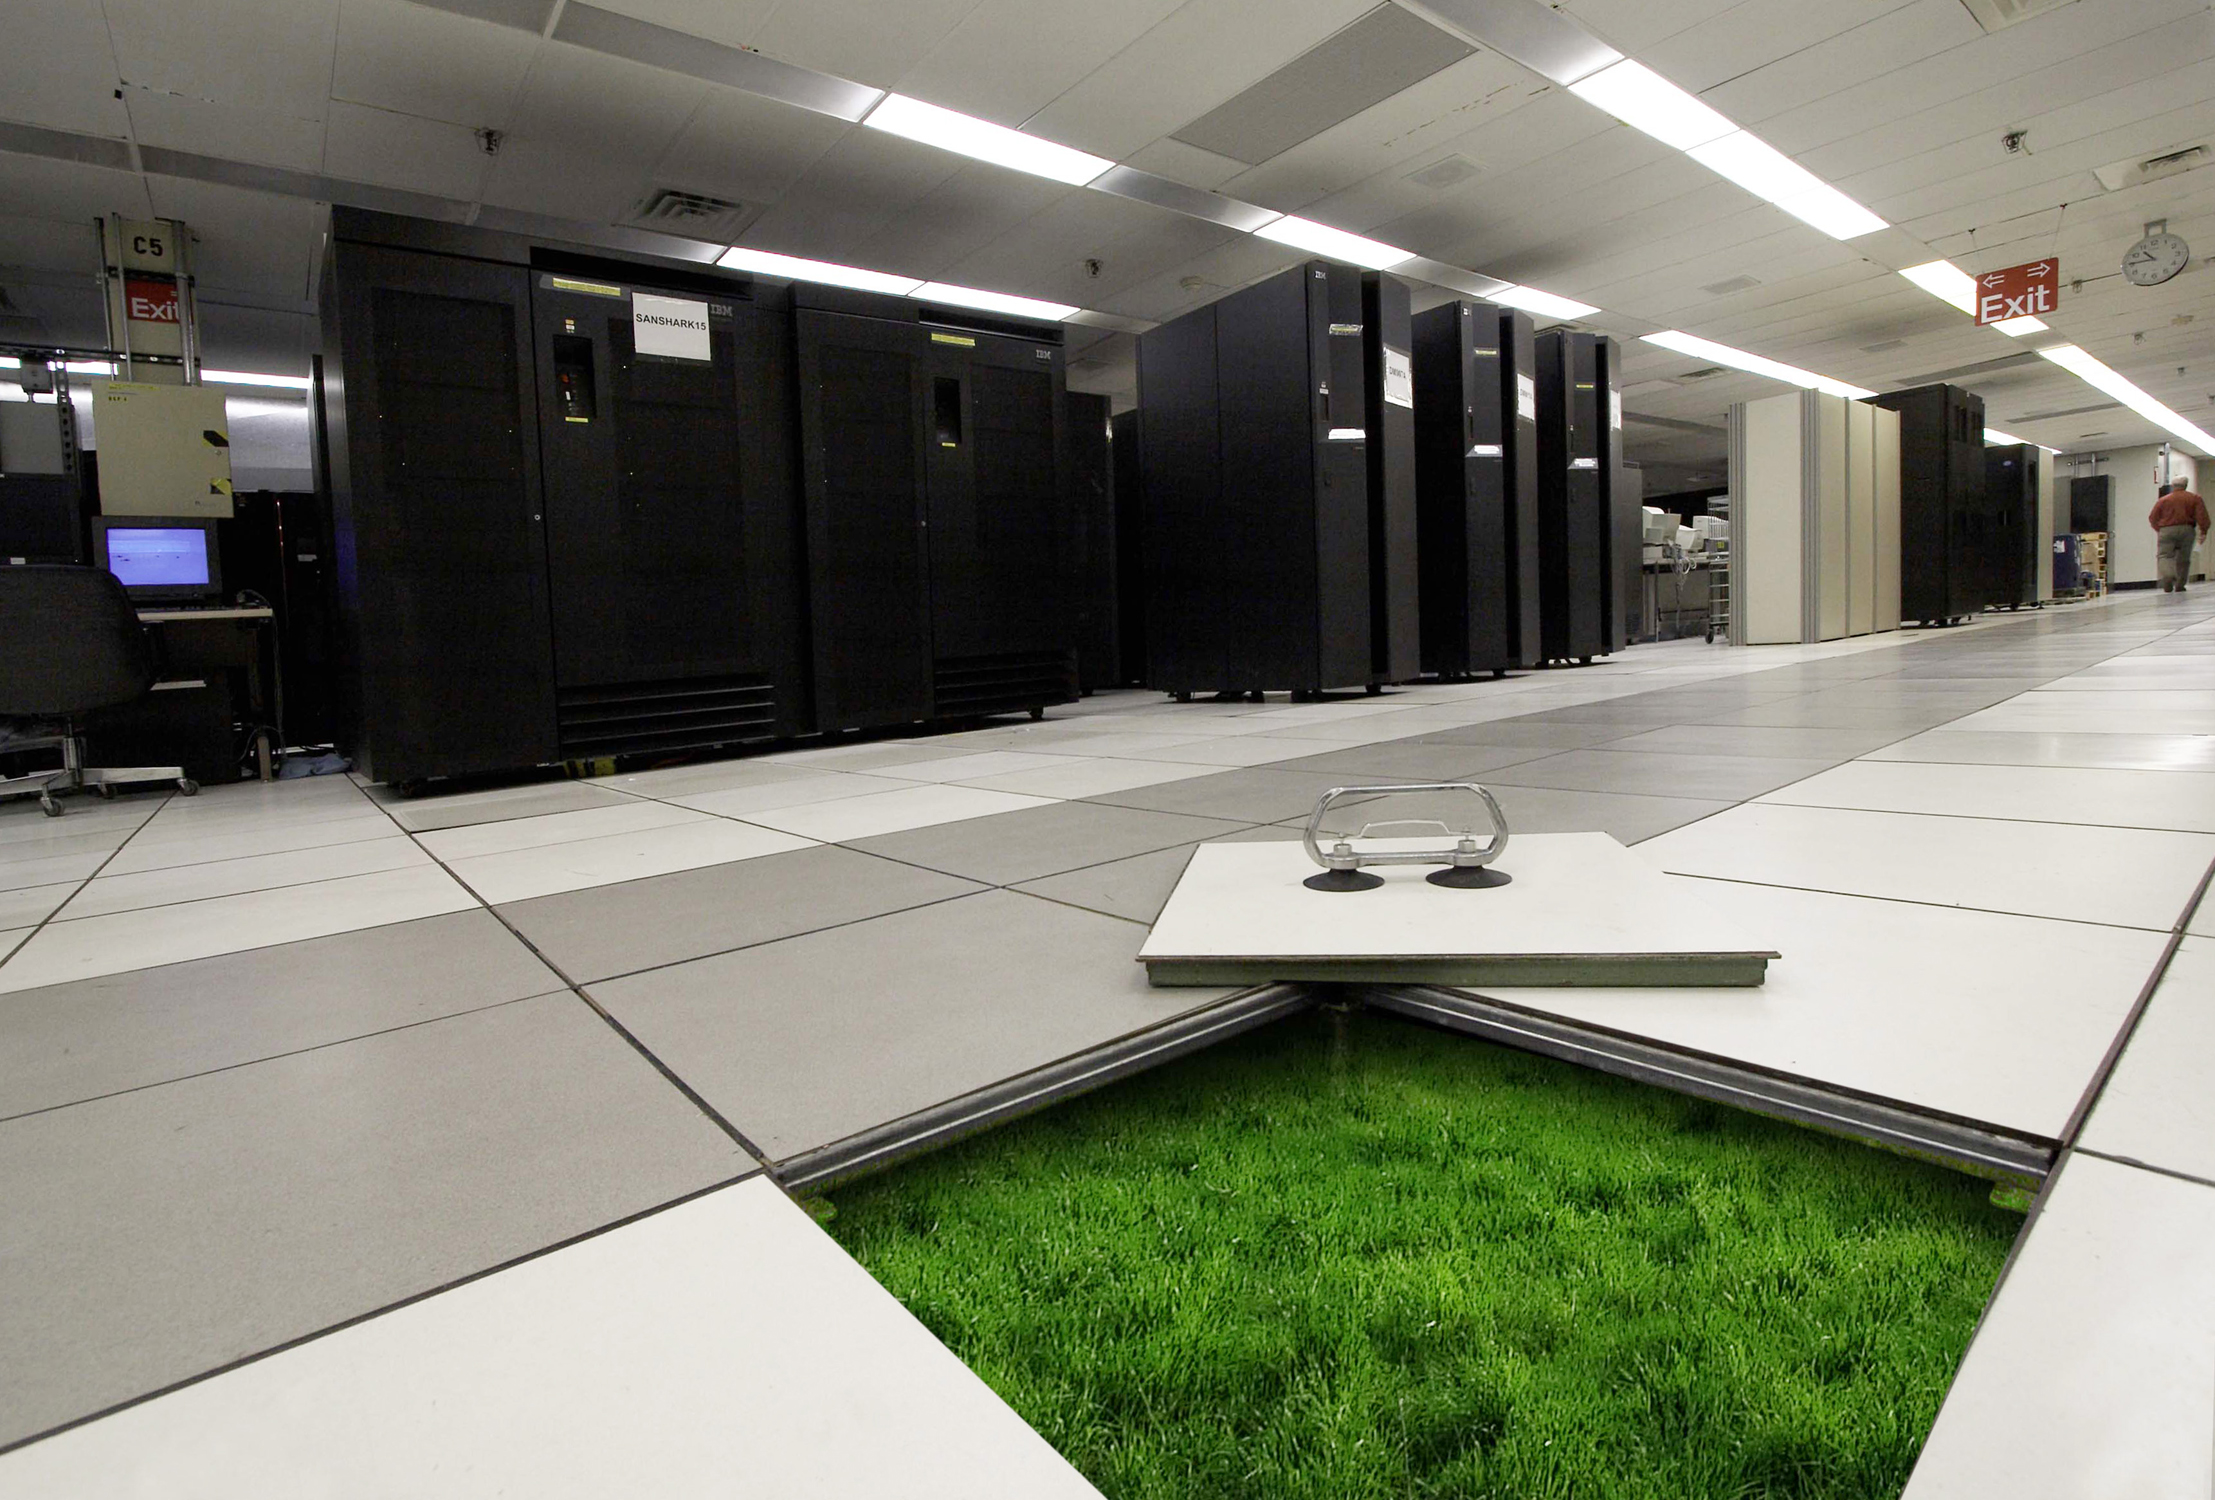
\includegraphics[height=\textwidth,angle=-90]{fig3}
%	\caption{Exemplo de figura rotacionada}
%	\label{fig3}
%\end{figure}

%\subsubsection{Resumo gráfico}

%Você pode optar por fazer um resumo no formato de mapa mental/conceitual. 
%Aqui foi utilizado o site https://app.mindmup.com para gerar o mapa.

%Para utilizar o resumo gráfico, remova o texto da seção resumo (linha 137) e inclua o código para inserir a figura, conforme figura \ref{fig4}

%\begin{table}[h!]
\centering
\caption{Exemplo de tabela explicativa}
\label{tab1}
\begin{tabular}{|l|l|l|}
\hline
\multicolumn{3}{|l|}{Figura na Tabela} \\ \hline
1        & Rack          & \includegraphics[scale=0.2]{fig1}        \\ \hline
2        & Rack 2        & \includegraphics[scale=0.2]{fig1}        \\ \hline
\end{tabular}
\end{table}

%\begin{figure}[h]
%	\centering
%	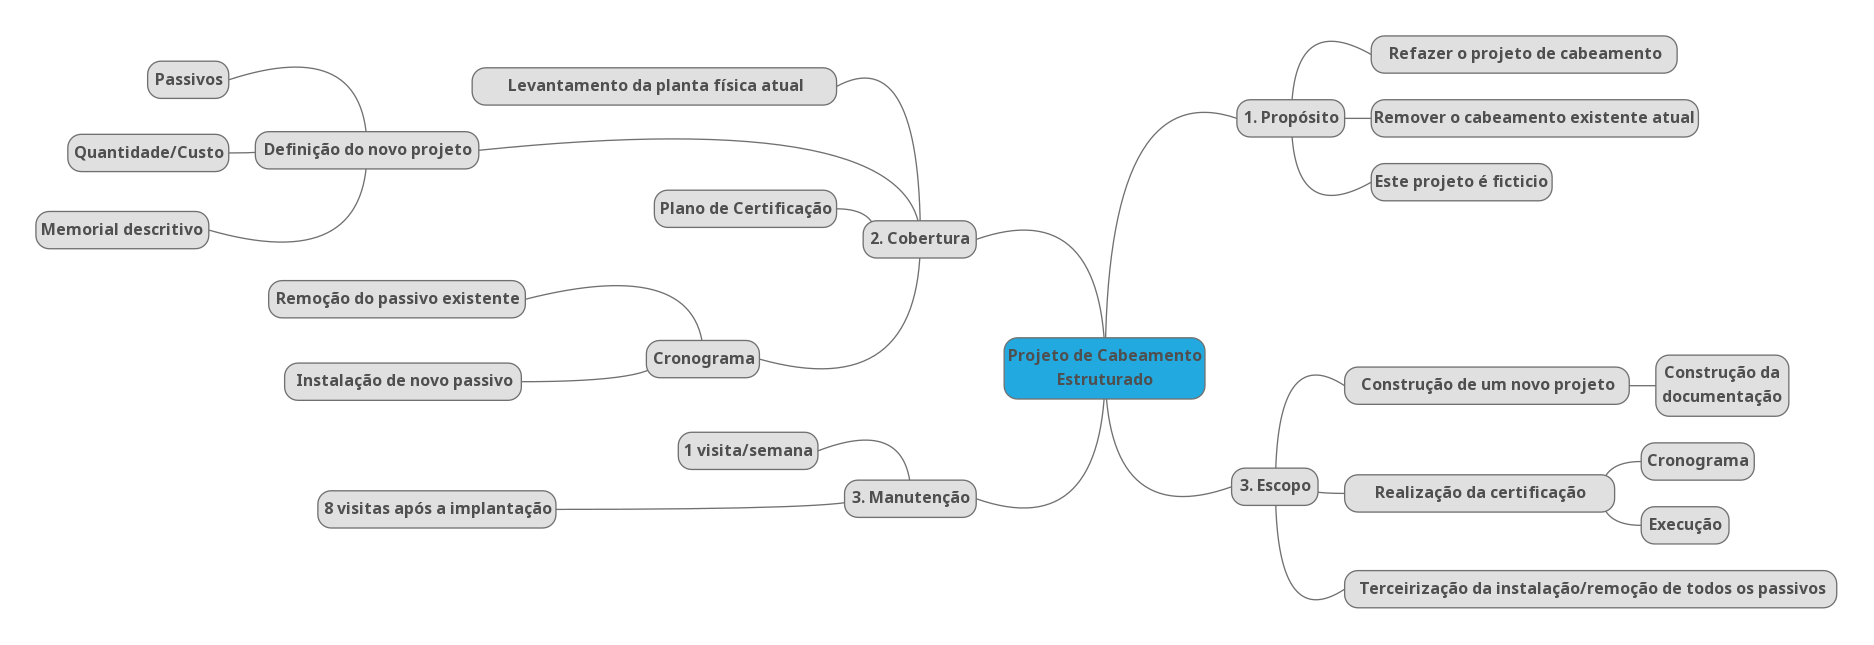
\includegraphics[width=\textwidth,height=5cm,keepaspectratio]{fig4}
%	\caption{Exemplo de resumo gráfico}
%	\label{fig4}	
%\end{figure}

%% ***********************************************************************
%% === ate aqui    =====  ================================================
%% ***********************************************************************

\end{document}